\documentclass[aps,pre,twocolumn,superscriptaddress,nofootinbib]{revtex4-2}
% preamble.tex -- paper K (revtex4-2, aps, pre, twocolumn); the macros of papers F, H, I and J where they are shared
\usepackage{amsmath,amssymb,amsthm,bm}
\usepackage{graphicx}
\usepackage{xcolor}
\raggedbottom   % no vertical stretching around headings when a float moves to the next page
\usepackage[colorlinks=true,linkcolor=black,citecolor=black,urlcolor=black]{hyperref}

% theorem environments (one counter)
\newtheorem{theorem}{Theorem}
\newtheorem{proposition}[theorem]{Proposition}
\newtheorem{lemma}[theorem]{Lemma}
\newtheorem{corollary}[theorem]{Corollary}
\newtheorem{conjecture}[theorem]{Conjecture}
\theoremstyle{definition}
\newtheorem{definition}[theorem]{Definition}
\theoremstyle{remark}
\newtheorem{remark}[theorem]{Remark}

% status labels (the spine of the paper)
\newcommand{\status}[1]{\textsf{[#1]}}
\newcommand{\proofst}{\status{proof}}
\newcommand{\caproofst}[1]{\status{proof, computer-assisted: #1}}
\newcommand{\derivst}{\status{derivation}}
\newcommand{\numst}{\status{numerical}}
\newcommand{\conjst}{\status{conjecture}}

% notation
\newcommand{\E}{\mathbb{E}}
\newcommand{\Jvv}{J_{vv}}
\newcommand{\Jww}{J_{ww}}
\newcommand{\keff}{k_{\mathrm{eff}}}
\newcommand{\kb}{\bar k}
\newcommand{\Lb}{\bar L}
\newcommand{\Var}{\operatorname{Var}}
\newcommand{\Cov}{\operatorname{Cov}}
\newcommand{\st}{\tilde s}
\newcommand{\Ht}{\tilde H}
\newcommand{\gaussk}{\mathcal N}
\newcommand{\Dc}{\mathcal D}
\newcommand{\Oset}{\mathcal O}
\newcommand{\Aw}{A_w}
\newcommand{\Nphi}{N_\varphi}
\newcommand{\BF}{B_{\mathrm F}}
\newcommand{\Wzz}{W_{zz}}
\newcommand{\hO}{h_{\mathcal O}}
\newcommand{\code}[1]{\texttt{#1}}
% DOIs
\newcommand{\Edoi}{10.5281/zenodo.23617343}
\newcommand{\Fdoi}{10.5281/zenodo.23746971}
\newcommand{\Fcodedoi}{10.5281/zenodo.23746555}
\newcommand{\Hdoi}{10.5281/zenodo.24369012}
\newcommand{\Idoi}{10.5281/zenodo.24371173}
\newcommand{\Icodedoi}{10.5281/zenodo.24370921}
\newcommand{\Jdoi}{10.5281/zenodo.24418628}
\newcommand{\Jcodedoi}{10.5281/zenodo.24418549}
% the code of this paper (the DOI is filled in at publication)
\newcommand{\Krepourl}{https://github.com/neginyan/resolution-gap-every-state}
\newcommand{\Kcodedoi}{[code DOI to be added]}


\begin{document}

% Paper K, version 1.0 (lab stage EI). Title: candidate 1 of stage EI (the main session decides; candidates in the report).
\title{\texorpdfstring{Every state keeps its arrow:\\ an unconditional lower bound on the resolution gap of the arrow of time}{Every state keeps its arrow: an unconditional lower bound on the resolution gap of the arrow of time}}

\author{Taishi Namba}
\email{neginyan@gmail.com}
\affiliation{Independent Researcher, Atsugi, Kanagawa, Japan}

\begin{abstract}
An observer sees a state of the pendulum near its upper equilibrium through Gaussian noise of width $\sigma$, and the resolution gap $g$ measures how much of the true expansion rate the blurred description loses.
It has been conjectured that $g$ never falls below $c'/\sqrt{\ell+C'}$, $\ell=\ln(1/\sigma)$, whatever the state; so far the lower side was known only for states built from a class of windows.
Here we prove a lower bound for every state, with no condition on its shape.
The only assumptions are a finite first moment and the confinement of the problem itself, $\Var(X_z)\le\pi^2$.
For every such state and every $\sigma\le1.5\times10^{-14}$,
\[
g\;\ge\;\frac{3}{4}\,\frac{\alpha}{\alpha\sigma+1268\,\kb},\qquad \kb^2=289\,\frac{\Lb^{5/2}}{(\ln2\Lb)^{3/2}}+4\Lb+3.57,
\]
with $\alpha=1/(2(\pi^2+\sigma^2))$ and $\Lb=2\ell+\ln(1/\alpha)$; for $\sigma\le10^{-15}$ this gives $g\ge1.7\times10^{-6}\,(\ln2\Lb)^{3/4}/\Lb^{5/4}$ \proofst.
The present power $\ell^{-5/4}(\ln\ell)^{3/4}$ is below the conjectured $\ell^{-1/2}$, the constants are small and the range of $\sigma$ is narrow; we state all three plainly.
Three steps carry the proof.
A three-circle argument in complex time bounds the second-order spread of the posterior for every state: $\keff^2\le289\,L^{5/2}/(\ln2L)^{3/2}+4L+3.57$ with $L=\ln(1/A)$, $A=\sigma^2\Jww$.
Outside an open set $\Oset$ where the $w$-information is of order $\sigma^2$, the remainder of the gap formula is at most half of its main terms.
Inside $\Oset$, an expansion of the gap around the observed point instead of the posterior mean has a remainder of order $\sigma^2\sqrt{\Jww+\Jvv}$, and the same complex-time argument in the isotropic flow controls the one second-order quantity left.
Every constant was recomputed with outward-rounded interval arithmetic, and every joint of the chain was evaluated on $6062$ recorded states without a failure \numst.
We state what is proved, derived and numerical, and what remains open: the power $\ell^{-1/2}$ and the range $\sigma>1.5\times10^{-14}$, with the inequality each rests on.

\end{abstract}

\maketitle

\section{Introduction}
\label{sec:intro}

How much of the arrow of time does an observer lose by looking at a system through a blur?
We ask this for the simplest unstable motion, the pendulum near its upper equilibrium, $\dot z=p$, $\dot p=\sin z$, which pulls nearby states apart at the rate $\kappa=1$.
The observer does not see the state $X$ itself, only $Y=X+\sigma Z$ with $Z\sim N(0,I_2)$: a Gaussian blur of width $\sigma$.
From the blurred density the observer reconstructs a drift through its score, and the rate $R$ that this drift reaches is smaller than $\kappa$.
The resolution gap $g=(\kappa-R)/\sigma$ measures the loss per unit of resolution (Sec.~\ref{sec:main} gives the precise definition).
The question is how small $g$ can become as the blur gets finer, and whether the answer depends on the state.

The natural candidate for a uniform answer is the logarithmic law
\begin{equation}
g\;\ge\;\frac{c'}{\sqrt{\ell+C'}},\qquad \ell=\ln(1/\sigma),
\label{eq:conj1}
\end{equation}
with constants $c',C'>0$ that do not depend on the state.
It was conjectured in Ref.~\cite{E}, where the weaker bound $g\ge c/\ell$ was proved for states without fine structure.
The law allows the gap to shrink as the blur gets finer, but only logarithmically, whatever the state.

So far the lower side of~\eqref{eq:conj1} was known only for states built from windows~\cite{F,H,I,J}.
A window is a smooth envelope that carries a periodic ripple in the stable direction of the equilibrium; the results cover weak and strong ripples and every place where the observer focuses.
A state that is not a window, for example one whose information sits in many scattered spots, was outside them.

This paper removes the shape.
Theorem~\ref{thm:main} gives a lower bound on $g$ for every probability measure on the plane with a finite first moment that is confined to the neighbourhood of the equilibrium, $\Var(X_z)\le\pi^2$.
The bound decays like $\ell^{-5/4}(\ln\ell)^{3/4}$.
That is slower than any power of $\sigma$, so the gap never closes at a finite resolution, but faster than the conjectured $\ell^{-1/2}$.
It holds for $\sigma\le1.5\times10^{-14}$, and its constant is small.
We regard the theorem as the first unconditional step towards~\eqref{eq:conj1}, and its power as the present one.
Section~\ref{sec:outlook} shows which inequality each of the next steps rests on: sharpening the power to $\ell^{-1/2}$, and widening the range of $\sigma$.

\paragraph*{Related work.}
That the arrow of time appears on the side of the coarse-grained description is a classical view~\cite{Lebowitz}.
The present problem is one concrete instance of it: the coarse-graining is a Gaussian blur of width $\sigma$, and the question is how much of the arrow it leaves, uniformly over the states.
A Gaussian blur moves the density along the heat flow, and how Fisher information behaves along that flow is the subject of de~Bruijn's identity and Stam's inequality~\cite{Stam}; for Gaussian channels, mutual information and the minimum mean-square error are related as well~\cite{GSV}.
The quantity $F(t)$ of Sec.~\ref{sec:circles}, the information in the stable direction along a heat flow in the unstable one, belongs to this family.
Tweedie's formula~\cite{Robbins,Efron}, which connects the posterior mean with the score, also underlies score-based estimation~\cite{Hyvarinen} and diffusion models~\cite{SongSDE}.
The central object of this paper, $\st=-\E[Z\mid Y]$, is exactly that score.
We use these connections as background only; the results of this paper concern the pendulum and the gap.

\paragraph*{What is new.}
Three steps make the shape irrelevant.
\begin{enumerate}
\item A bound on the effective wavenumber, $\keff^2\le\psi(\ln(1/A))$ with $\psi(L)=289L^{5/2}/(\ln2L)^{3/2}+4L+3.57$, for every state (Theorem~\ref{thm:circles}).
Earlier proofs needed such a bound and had it only as a conjecture or for windows.
The proof goes through complex time: the stable-direction score of the density with $v$-noise $z$ is a holomorphic function of $z$ with values in a Hilbert space, and Hadamard's three-circle theorem transports its smallness at $z=1$ to $z$ slightly below one.
The three-circle argument was proposed by Google Gemini, one of the AI assistants used in this work (see the Acknowledgments), and checked here line by line and numerically at every step.
\item A threshold for the remainder of the gap formula of Ref.~\cite{E}: once the $w$-information and the curved $v$-information together exceed $112\sigma^2$, the remainder is at most half of the main terms (Lemma~\ref{lem:EF2}).
So every remainder estimate is needed only on an open set $\Oset$ of states with information of order $\sigma^2$.
\item On $\Oset$ the gap is expanded around the observed point $Y_z$ instead of the posterior mean $m_z$ (Lemma~\ref{lem:EGD}).
The state-independent remainder $(\sqrt{960}/6)\sigma^2$ of the old expansion disappears; the new remainder carries $\sqrt{A+B}$, and the single second-order quantity left, $\Wzz=\sigma^2\partial_z^2\varrho/\varrho$, is controlled by the same three circles in the isotropic flow (Lemmas~\ref{lem:iso} and~\ref{lem:sm}).
\end{enumerate}
The rest of the chain is borrowed from Refs.~\cite{E,F} and from the lab stages behind this paper; Section~\ref{sec:chain} shows how it fits together, and the appendices state every borrowed lemma in the notation used here.

\paragraph*{How the results are checked.}
Every statement carries one of the labels \proofst, \derivst, \numst\ or \conjst.
There is no computer-assisted step in the proof of Theorem~\ref{thm:main}: every constant is a closed form.
We nevertheless recomputed all of them with outward-rounded interval arithmetic (App.~\ref{app:constants}), and we evaluated every joint of the chain, the conclusion of one lemma inserted into the hypothesis of the next, on $6062$ recorded states (App.~\ref{app:joints}).
That check found three printed rounded values whose direction was wrong in the working record; the constants derived from them hold when recomputed.
It also reproduces, as a deliberately wrong version, an earlier slip in a power of $\sigma$, which fails by a factor of $9\times10^{71}$.

\paragraph*{Plan.}
We refer to Refs.~\cite{E}, \cite{F} and~\cite{H,I,J} as Papers~E, F, H, I and~J, the names used in the code and the records.
Section~\ref{sec:main} states the setting and Theorem~\ref{thm:main}.
Section~\ref{sec:chain} shows the chain.
Sections~\ref{sec:circles}--\ref{sec:inside} prove the three new steps, and Section~\ref{sec:assembly} assembles the proof and discusses the range of $\sigma$.
Section~\ref{sec:outlook} lists what remains between Theorem~\ref{thm:main} and the conjecture~\eqref{eq:conj1}.

\section{Setting and main result}
\label{sec:main}

\subsection{The state, the observer and the gap}
A \emph{state} is a probability measure $\rho$ on $\mathbb R^2$; $X\sim\rho$.
We assume
\begin{equation}
\text{(M1)}\quad \E|X|<\infty,\qquad\qquad \text{(H2)}\quad \Var(X_z)\le\pi^2 .
\label{eq:assumptions}
\end{equation}
No density is required.
The observer sees $Y=X+\sigma Z$ with $Z\sim N(0,I_2)$ independent of $X$ and $\sigma>0$; we write $Z=(Y-X)/\sigma$ throughout.
The blurred density is $\varrho=\rho*N(0,\sigma^2 I)$ (we keep $p$ for a coordinate), and $\E$ is the expectation over $Y\sim\varrho$.
Coordinates $(v,w)$ are the unstable and stable directions of the pendulum at its upper equilibrium, and
$z=(v+w)/\sqrt2$, $p=(v-w)/\sqrt2$.
(H2) is part of the problem: the observer looks at the neighbourhood of the equilibrium, one period of the pendulum in $z$.

With the score $s=\nabla\ln\varrho$ and $f(x)=(x_p,\sin x_z)$ in the $(z,p)$ components, the critical rate and the gap of Paper~E are
\begin{equation}
R=\frac{\E\big[s\cdot\E[f(X)\mid Y]\big]}{\sigma^2\E|s|^2},\qquad g=\frac{1-R}{\sigma}.
\end{equation}

\paragraph*{Dimensionless quantities.}
$\st=\sigma s=-\E[Z\mid Y]$ and $\Ht=-\sigma^2\nabla^2\ln\varrho=I-\Cov(Z\mid Y)$ (Tweedie, Lemma~\ref{lem:tweedie}).
\begin{equation}
A=\sigma^2\Jww=\E[\st_w^2],\quad B=\sigma^2\Jvv=\E[\st_v^2],\quad J=A+B .
\end{equation}
With the posterior mean $m=\E[X\mid Y]$ and $\varphi=1-\cos m_z$, let $\theta=\E[\st_v^2\varphi]/B$ and
\begin{equation}
M=A+\tfrac12\theta B,\qquad \Oset=\{M<112\,\sigma^2\}.
\label{eq:Oset}
\end{equation}
The effective wavenumber of Paper~F is $\keff^2=\sigma^2\int(\partial_v\partial_w\sqrt\varrho)^2/\int(\partial_w\sqrt\varrho)^2$; in dimensionless form $\keff^2=K/A$ with $K=\E[(\partial_v\st_w+\tfrac12\st_v\st_w)^2]$ (Lemma~\ref{lem:K}).
Finally $\ell=\ln(1/\sigma)$, $\alpha=1/(2(\pi^2+\sigma^2))$ and
\begin{equation}
\begin{gathered}
\psi(L)=289\,\frac{L^{5/2}}{(\ln2L)^{3/2}}+4L+3.57,\\ \Lb=2\ell+\ln\frac1\alpha,\qquad \kb=\sqrt{\psi(\Lb)} .
\end{gathered}
\label{eq:psi}
\end{equation}

\subsection{The main theorem}

\begin{theorem}[Every state keeps a gap]\label{thm:main}
Let $\rho$ satisfy \textup{(M1)} and \textup{(H2)}, and let $c_r=\sqrt{0.1}$.
\begin{enumerate}
\item[(a)] If $0<\sigma\le10^{-4}$ and $M\ge112\sigma^2$, then
\[
g\ \ge\ \min\Big\{1,\ \frac{c_r}{2\sqrt\ell},\ 0.14(1-2\sigma),\ \frac{(1-2\sigma)(1-0.284)}{4\sqrt2\,\kb}\Big\}.
\]
\item[(b)] If $0<\sigma\le1.5\times10^{-14}$, then for every state
\[
g\ \ge\ \frac34\,\frac{\alpha}{\alpha\sigma+1268\,\kb},
\]
and this is the smallest of the five lower bounds of (a) and (b).
\item[(c)] If $0<\sigma\le10^{-15}$, then for every state
\[
g\ \ge\ \frac{2.9\times10^{-5}}{\kb}\ \ge\ 1.7\times10^{-6}\,\frac{(\ln2\Lb)^{3/4}}{\Lb^{5/4}} .
\]
\end{enumerate}
\proofst
\end{theorem}

The proof is assembled in Section~\ref{sec:assembly}.
At $\sigma=10^{-15}$ one has $\Lb=72.06$ and $\kb=1072.3$, so the bound of (b) is $2.79\times10^{-8}$.
As $\sigma\to0$, $\kb\sim17\,\Lb^{5/4}/(\ln2\Lb)^{3/4}$ and $\Lb\sim2\ell$, so (c) reads $g\ge c'(\ln\ell)^{3/4}/\ell^{5/4}$.

\begin{remark}[What the theorem does not say]\label{rem:limits}
The power $5/4$ is larger than the conjectured $1/2$ of~\eqref{eq:conj1}; it comes from the factor $L^{5/2}$ in $\psi$.
The constant is small, and the range $\sigma\le1.5\times10^{-14}$ is narrow.
For $10^{-14}\lesssim\sigma\le10^{-4}$ part (a) still covers every state outside $\Oset$; inside $\Oset$ the theorem says nothing there.
We state these limits because they are exactly what the next steps must improve (Section~\ref{sec:outlook}), not because the result is conditional: within its range, it holds for every state.
\end{remark}

\subsection{In the observer's words}
The observer cannot choose the state.
It may be smooth or rough, concentrated on a few points or spread over the whole neighbourhood, with fine structure in one direction and none in the other.
Whatever it is, the observer's reconstruction of the unstable motion stays measurably slower than the true motion.
The loss per unit of resolution, $g$, shrinks as the lens sharpens, but only like a power of $\ln(1/\sigma)$, never like a power of $\sigma$.
Three facts carry this.
A state cannot hide its fine structure from a slightly blurrier lens: when the $v$-noise is lowered a little, the information about the stable direction grows by at most a polynomial in $\ln(1/A)$ (Theorem~\ref{thm:circles}).
When the information is not small, the error of the observer's formula is at most half of what it explains.
And when the information is small, the observer should read the motion at the point it sees rather than at the point it infers; there the error is proportional to the information itself.

\section{The chain}
\label{sec:chain}

Figure~\ref{fig:chain} shows how Theorem~\ref{thm:main} rests on its parts.
Table~\ref{tab:chain} lists them in the order of use, with their origin and their units.

\begin{figure*}[t]
\centering
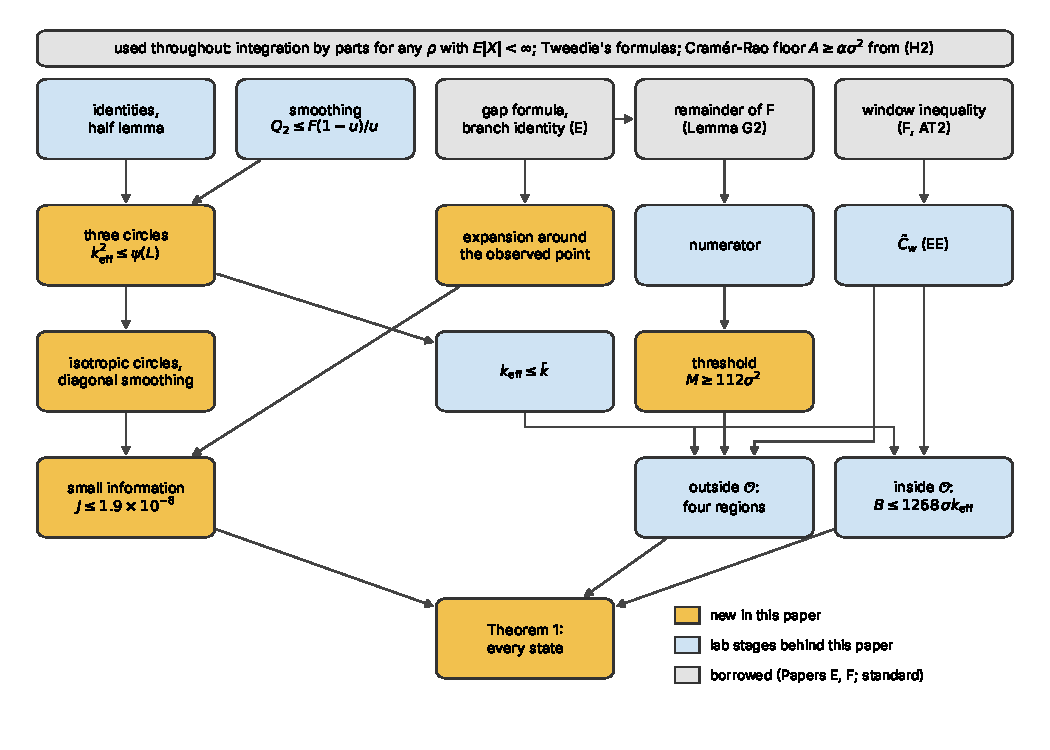
\includegraphics[width=0.8\textwidth]{figures/fig_chain_K.pdf}
\caption{The chain of Theorem~\ref{thm:main}. Boxes are the results of this paper and the borrowed ones (grey); an arrow means ``is used by''. The three new steps are Theorem~\ref{thm:circles} (three circles), Lemma~\ref{lem:EF2} (the threshold that confines every remainder estimate to $\Oset$) and Lemma~\ref{lem:EGD} with Theorem~\ref{thm:EGO} (the expansion around the observed point).}
\label{fig:chain}
\end{figure*}

\begin{table*}[t]
\caption{The parts of the chain in the order of use. Units: ``raw'' are formulas in the original coordinates, ``dimensionless'' are formulas in $\st$, $\Ht$ with $\sigma$ written explicitly, and ``$\sigma=1$'' are formulas for the state $X/\sigma$ with unit noise. Origin: E, F are Papers~E and~F; ED--EH are the lab stages behind this paper; G marks steps proposed by Google Gemini, one of the AI assistants used in this work (see the Acknowledgments).}
\label{tab:chain}
\begin{ruledtabular}
\begin{tabular}{lll}
part & origin & units\\
\hline
Lemma~\ref{lem:ibp} (integration by parts) & EF, EG & raw\\
Lemma~\ref{lem:tweedie} (Tweedie) & standard~\cite{Efron,Robbins} & raw/dimensionless\\
Proposition~\ref{prop:gap} (gap formula) & E, EG & dimensionless\\
Proposition~\ref{prop:branch} (branch identity) & E & dimensionless\\
Lemma~\ref{lem:G2} (remainder of F) & F & raw\\
Lemma~\ref{lem:EF1} (numerator) & EF, G & dimensionless\\
Lemma~\ref{lem:EF2} (threshold) & EF & dimensionless\\
Lemma~\ref{lem:CR} (Cram\'er--Rao floor) & E, EE & dimensionless\\
Lemma~\ref{lem:K} (identities, half lemma) & ED, EF, G & $\sigma=1$\\
Lemma~\ref{lem:smooth} (smoothing) & EF & $\sigma=1$\\
Lemmas~\ref{lem:kernel}--\ref{lem:holo} (circles) & EG, G & $\sigma=1$\\
Theorem~\ref{thm:circles} ($\keff^2\le\psi$) & EG, G & $\sigma=1$\\
Lemma~\ref{lem:window} (window inequality) & F, EE, EF & raw$\to$dimensionless\\
Lemma~\ref{lem:EEC} ($\tilde C_w$) & EE & dimensionless\\
Lemma~\ref{lem:EFO} (inside $\Oset$) & EF & dimensionless\\
Proposition~\ref{prop:outside} (outside $\Oset$) & EF & dimensionless\\
Lemma~\ref{lem:EGD} (direct expansion) & EG & dimensionless\\
Lemmas~\ref{lem:iso},~\ref{lem:sm} (isotropic) & EG, G & $\sigma=1$\\
Theorem~\ref{thm:EGO} (small information) & EG & dimensionless\\
Theorem~\ref{thm:main} & EG, EH, EI & dimensionless
\end{tabular}
\end{ruledtabular}
\end{table*}

Two remarks on the joints.
First, the powers of $\sigma$ change at four places: the Lagrange remainder of Lemma~\ref{lem:G2} (a factor $\sigma^2$), the window inequality (the $\sigma^{-2}$ of $\int(\partial_wf)^2=\keff^2\Jww/\sigma^2$, Lemma~\ref{lem:window}), the bound $B\le\sigma\cdots$ inside $\Oset$ (Lemma~\ref{lem:EFO}), and the remainders $\sigma^2\sqrt J$ and $\sigma\,\Wzz$ of Lemma~\ref{lem:EGD}.
Each of them is checked numerically on recorded states (App.~\ref{app:joints}); the window inequality without its factor $\sigma^2$, which appeared once in the working record, fails there by a factor of $9\times10^{71}$.
Second, the assumptions travel as follows: (M1) enters only through Lemma~\ref{lem:ibp}(ii), used by the gap formula and the branch identity; (H2) enters only through the Cram\'er--Rao floor, $A\ge\alpha\sigma^2$, from which $\ln(1/A)\le\Lb$ and $\keff\le\kb$.
Paper~F's Lemma~BB1 and the ``sufficient decay'' assumed in Papers~E and~F are not used.

\section{The effective wavenumber of every state}
\label{sec:circles}

Throughout this section we use units $\sigma=1$: $\tilde\rho$ is the law of $X/\sigma$ and the noise is $N(0,I_2)$.
For $\operatorname{Re}t>0$ let $\gaussk_t(u)=(2\pi t)^{-1/2}e^{-u^2/(2t)}$ (principal square root), and
\begin{equation}
\varrho_t(v,w)=\int\gaussk_t(v-x_v)\,\gaussk_1(w-x_w)\,d\tilde\rho(x),\qquad q_t=\partial_w\varrho_t ,
\end{equation}
the density with $v$-noise of variance $t$ and $w$-noise of variance one.
For $t>0$ let $F(t)=\int q_t^2/\varrho_t$ be the $w$-information at $v$-noise $t$; then $F(1)=A$, and we write $L=\ln(1/A)$.
With $Q_2=\E[(\E[Z_vZ_w\mid Y])^2]$, $\mathrm{SV}=\E[\st_w^2\Var(Z_v\mid Y)]$ and $\mathrm{S2}=\E[\st_v^2\st_w^2]$:

\begin{lemma}[Identities and the half lemma]\label{lem:K}
For every state,
$K=Q_2+\tfrac12\mathrm{SV}-\tfrac12A-\tfrac14\mathrm{S2}\le Q_2+\tfrac12\mathrm{SV}$, and $\mathrm{SV}\le8AL+7.136A$.
\proofst\ (App.~\ref{app:borrowed}.)
\end{lemma}

\begin{lemma}[Smoothing]\label{lem:smooth}
For every state and every $u\in(0,1)$, $Q_2\le F(1-u)/u$.
\end{lemma}
\begin{proof}\proofst\
Split $Z_v=\sqrt{1-u}\,Z_1+\sqrt u\,Z_2$ with $Z_1,Z_2$ independent standard normal, and let $Y'=(X_v+\sqrt{1-u}Z_1,\,Y_w)$, whose density is $\varrho_{1-u}$; then $Y=Y'+(\sqrt uZ_2,0)$.
Since $(Z_1,Z_2)$ is independent of $(X,Z_w)$, $\E[Z_2\mid X,Z_w,Z_v]=\sqrt u\,Z_v$, and the tower property gives $\E[Z_2Z_w\mid Y]=\sqrt u\,\E[Z_vZ_w\mid Y]$.
Since $Y$ is a function of $(Y',Z_2)$ and $Z_2$ is independent of $(X,Z_1,Z_w)$, also $\E[Z_2Z_w\mid Y]=\E[Z_2\,h(Y')\mid Y]$ with $h(y')=\E[Z_w\mid Y'=y']=-\partial_w\ln\varrho_{1-u}(y')$.
By Jensen and $Z_2\perp Y'$, $Q_2\le u^{-1}\E[Z_2^2]\,\E[h(Y')^2]=F(1-u)/u$.
\end{proof}

So $\keff^2$ is controlled once $F$ cannot grow fast when the $v$-noise is lowered from $1$ to $1-u$.
For a general state $F(1-u)$ can exceed $F(1)$ by a large factor, but not when $u$ is small compared with $1/\ln(1/A)$.
The tool is Hadamard's three-circle theorem~\cite{Conway,Titchmarsh} in the Hilbert space $H_T=L^2(dy/\varrho_T)$.
The argument was proposed by Google Gemini, one of the AI assistants used in this work (see the Acknowledgments); we give it with its constants and with the integrability it needs.

\begin{lemma}[Kernel integrals]\label{lem:kernel}
Let $T>0$ and $|z-T|=r<T$. Then $\int|\gaussk_z|^2/\gaussk_T\,du=(1-(r/T)^2)^{-1/2}$ and $\int u^2|\gaussk_z|^2/\gaussk_T\,du=(1-(r/T)^2)^{-1/2}\,T|z|^2/(T^2-r^2)$.
\end{lemma}
\begin{proof}\proofst\
$|\gaussk_z(u)|^2=(2\pi|z|)^{-1}e^{-u^2\operatorname{Re}z/|z|^2}$, so $|\gaussk_z|^2/\gaussk_T=\frac{\sqrt T}{\sqrt{2\pi}|z|}\exp\!\big(-u^2\frac{2T\operatorname{Re}z-|z|^2}{2T|z|^2}\big)$.
For $z=T+re^{i\vartheta_0}$, $2T\operatorname{Re}z-|z|^2=T^2-r^2$ for every angle; both integrals are Gaussian with variance $T|z|^2/(T^2-r^2)$.
\end{proof}

\begin{lemma}[Outer and inner circles]\label{lem:circles}
(i) If $|z-T|=r<T$, then $\|q_z\|^2_{H_T}\le(1-(r/T)^2)^{-1/2}$.
(ii) If $T=1+\delta$ and $|z-T|=r<\delta$, then $\|q_z\|^2_{H_T}\le A\,(1-(r/\delta)^2)^{-1/2}$.
\end{lemma}
\begin{proof}\proofst\
(i) $q_z(y)=-\int\gaussk_z(v-x_v)(w-x_w)\gaussk_1(w-x_w)\,d\tilde\rho(x)$.
Cauchy--Schwarz in $\tilde\rho$ with the weight $\sqrt{\gaussk_T\gaussk_1}$ gives $|q_z|^2\le\varrho_T\int(|\gaussk_z|^2/\gaussk_T)(v-x_v)\,(w-x_w)^2\gaussk_1(w-x_w)\,d\tilde\rho$; divide by $\varrho_T$, integrate in $y$ (Tonelli), and use $\int w'^2\gaussk_1=1$ and Lemma~\ref{lem:kernel}.
(ii) $\operatorname{Re}(z-1)\ge\delta-r>0$.
The semigroup law $\gaussk_{a+b}=\gaussk_a*\gaussk_b$ holds for $\operatorname{Re}a,\operatorname{Re}b>0$ (both sides are holomorphic in $a$ and agree for real $a$), so $q_z=\gaussk_{z-1}*_vq_1$ and $\varrho_T=\gaussk_\delta*_v\varrho_1$.
For fixed $w$, Cauchy--Schwarz in $v'$ with the weight $\gaussk_\delta(v-v')\varrho_1(v',w)$ gives $|q_z|^2\le\varrho_T\int(|\gaussk_{z-1}|^2/\gaussk_\delta)(v-v')\,q_1^2/\varrho_1\,dv'$; divide, integrate, and use Lemma~\ref{lem:kernel} for $(\delta,z-1)$ and $\int q_1^2/\varrho_1=A$.
\end{proof}

\begin{lemma}[Holomorphy and three circles]\label{lem:holo}
Let $\mathfrak D=\{|z-T|<T\}$.
(i) For each $\chi\in H_T$, $f_\chi(z)=\int\bar\chi\,q_z/\varrho_T\,dy$ is holomorphic on $\mathfrak D$.
(ii) If $0<r_1<r_2<r_3<T$ and $|z_2-T|=r_2$, then $\|q_{z_2}\|\le(\sup_{|z-T|=r_1}\|q_z\|)^{1-\vartheta}(\sup_{|z-T|=r_3}\|q_z\|)^{\vartheta}$ with $\vartheta=\ln(r_2/r_1)/\ln(r_3/r_1)$.
\end{lemma}
\begin{proof}\proofst\
(i) Let $\mathcal K\subset\mathfrak D$ be compact.
On $\mathcal K$, $r=|z-T|\le r_{\mathcal K}<T$ and $|z|$ lies between two positive constants, so by the formula in the proof of Lemma~\ref{lem:kernel},
\[
|\gaussk_z(u)|^2/\gaussk_T(u)\le C_{\mathcal K}\,e^{-c_{\mathcal K}u^2},\qquad c_{\mathcal K}=\min_{\mathcal K}\frac{T^2-r^2}{2T|z|^2}>0 .
\]
Let $G_{\mathcal K}(y)=C_{\mathcal K}\int e^{-c_{\mathcal K}(v-x_v)^2}(w-x_w)^2\gaussk_1(w-x_w)\,d\tilde\rho(x)$; it does not depend on $z$, and $\int G_{\mathcal K}\,dy=C_{\mathcal K}\sqrt{\pi/c_{\mathcal K}}<\infty$.
The Cauchy--Schwarz step of Lemma~\ref{lem:circles}(i) gives $|q_z|^2\le\varrho_TG_{\mathcal K}$ for every $z\in\mathcal K$, hence
\[
\begin{gathered}
|\bar\chi\,q_z/\varrho_T|\le(|\chi|/\sqrt{\varrho_T})\sqrt{G_{\mathcal K}}\in L^1,\\ \sup_{z\in\mathcal K}\|q_z\|_{H_T}^2\le\|G_{\mathcal K}\|_{L^1}.
\end{gathered}
\]
For each $y$, $z\mapsto q_z(y)$ is holomorphic on $\operatorname{Re}z>0$ (the integrand is holomorphic in $z$ and bounded on compact sets uniformly in $x$), so $\oint_{\partial\Delta}q_z(y)\,dz=0$ for every triangle $\Delta\subset\mathfrak D$ by Cauchy's theorem.
By the dominating function and Fubini, $\oint_{\partial\Delta}f_\chi\,dz=\int(\bar\chi/\varrho_T)\oint_{\partial\Delta}q_z\,dz\,dy=0$, and $f_\chi$ is continuous by dominated convergence; Morera's theorem gives (i).
(ii) Hadamard's three-circle theorem for $f_\chi$ with $\|\chi\|=1$, $|f_\chi(z)|\le\|q_z\|$, and the supremum over $\chi$.
\end{proof}

\begin{theorem}[The effective wavenumber of every state]\label{thm:circles}
Let $A\le e^{-4}$, $L=\ln(1/A)$, and
\[
\begin{gathered}
\delta=\tfrac1{4L},\quad T=1+\delta,\quad \eta=\tfrac{\ln2L}{4L},\quad \tau=\tfrac{\ln2L}{8L^2},\\ r_1=\delta(1-\eta),\quad r_2=\delta+\tau,\quad r_3=\tfrac T2 .
\end{gathered}
\]
Then
(i) $\|q_{1-\tau}\|^2_{H_T}\le\frac{4e}{\sqrt3}\sqrt{L/\ln2L}\;A$;
(ii) $F(1-\tau)\le36.1\sqrt{L/\ln2L}\;A$;
(iii) $Q_2\le289\,A\,L^{5/2}/(\ln2L)^{3/2}$;
(iv) $\keff^2\le\psi(L)$.
(v) If $A>e^{-4}$, $\keff^2\le74.2\le\psi(4)$.
So \emph{every} state has $\keff^2\le\psi(\max(\ln(1/A),4))$.
\end{theorem}
\begin{proof}\proofst\
\emph{Numbers.} For $L\ge4$: $\eta\le0.12997$, $\tau\le0.016246$, $\delta\le1/16$ (all decrease in $L$), so $r_1<r_2<r_3<T$, the point $1-\tau$ lies on the circle $|z-T|=r_2$, and $\operatorname{Re}z\ge T/2$ on $|z-T|\le r_3$.
\emph{Circles.} Lemma~\ref{lem:circles}(i) with $r=T/2$ gives $\sup\|q_z\|^2\le2/\sqrt3$ on the outer circle; Lemma~\ref{lem:circles}(ii) with $r=r_1$ gives $\le A/\sqrt{2\eta-\eta^2}\le A/\sqrt\eta$ on the inner circle.
\emph{The exponent.} $r_3/r_1=2L(1+\delta)/(1-\eta)>2L$, and $\ln(r_2/r_1)=\ln(1+\tau/\delta)-\ln(1-\eta)\le\tau/\delta+2\eta=\ln(2L)/L$ (for $\eta\le0.13$, $-\ln(1-\eta)\le2\eta$); so $\vartheta<1/L$.
\emph{(i).} By Lemma~\ref{lem:holo}, $\|q_{1-\tau}\|^2\le(A/\sqrt\eta)^{1-\vartheta}(2/\sqrt3)^{\vartheta}\le e\,A\,\eta^{-1/2}\,2/\sqrt3$, since $A^{-\vartheta}=e^{\vartheta L}<e$; and $\eta^{-1/2}=2\sqrt{L/\ln2L}$.
\emph{Back to the weight $1/\varrho_{1-\tau}$.} With $u=\sqrt T\zeta$, $\gaussk_{1-\tau}(u)/\gaussk_T(u)=c_Te^{-\omega\zeta^2}$, where $c_T=\sqrt{T/(1-\tau)}$ and $\omega=(\tau+\delta)/(2(1-\tau))$.
Hence, exactly, $\varrho_{1-\tau}=c_T\varrho_TW_T$ and $q_{1-\tau}=-c_T\varrho_T\E[Z_we^{-\omega Z_v^2}\mid Y_T]$, with $W_T(y)=\E[e^{-\omega Z_v^2}\mid Y_T=y]$, $Y_T=(X_v+\sqrt TZ_v,X_w+Z_w)$.
For $L\ge4$, $\omega<1/(4L)$, since this is equivalent to $\ln(2L)(1+1/(2L))<2L$.
Let $K_b^2=4L$, so $\omega K_b^2<1$, and $E_{\rm bad}=\{W_T<1/(2e)\}$.
As $W_T\ge e^{-\omega K_b^2}P(|Z_v|\le K_b\mid y)>e^{-1}P(|Z_v|\le K_b\mid y)$, on $E_{\rm bad}$ one has $P(|Z_v|>K_b\mid y)>\frac12$, and Markov's inequality gives $P_T(E_{\rm bad})\le2P(|Z_v|>K_b)\le2e^{-2L}=2A^2$.
The conditional Cauchy--Schwarz inequality gives $q_{1-\tau}^2/\varrho_{1-\tau}\le c_T\varrho_T\E[Z_w^2\mid Y_T]$ at every $y$, so the contribution of $E_{\rm bad}$ to $F(1-\tau)$ is at most $c_T\sqrt{2A^2}\sqrt{\E Z_w^4}=\sqrt{6T/(1-\tau)}\,A\le2.55A$.
Outside $E_{\rm bad}$, $\varrho_{1-\tau}\ge c_T\varrho_T/(2e)$ and $c_T>1$, so the contribution is at most $2e\|q_{1-\tau}\|^2_{H_T}\le34.13\sqrt{L/\ln2L}\,A$.
Since $\sqrt{L/\ln2L}$ increases and is $1.38693\ldots$ at $L=4$, the sum is at most $36.1\sqrt{L/\ln2L}\,A$; this is (ii).
\emph{(iii)} is Lemma~\ref{lem:smooth} with $u=\tau$, $1/\tau=8L^2/\ln2L$ and $36.1\cdot8\le289$.
\emph{(iv)} follows from Lemma~\ref{lem:K}: $\keff^2=K/A\le Q_2/A+4L+3.568$.
\emph{(v)} Jensen gives $Q_2\le\E[Z_v^2Z_w^2]=1$, so $Q_2/A<e^4$, and $\frac12\mathrm{SV}/A<19.57$ for $L<4$; $e^4+19.57<74.17\le\psi(4)=3103.7$, and $\psi$ increases on $[4,\infty)$.
\end{proof}

\begin{remark}[The choice of $\delta$]\label{rem:delta}
$\delta=1/(4L)$ is one sufficient choice, not a forced one.
The return step needs only $\omega K_b^2<1$; for instance $\delta=0.4/L$ gives $\omega K_b^2=(0.8+\ln(2L)/(4L))/(1-\tau)=0.9453$ at $L=4$ \proofst, with other constants.
We have not optimized the choice.
What the argument does need is that $\delta\ln(1/A)$ stays bounded: a $v$-noise of order one would fill the valleys of $\varrho_1$ and the weight $1/\varrho_T$ could not be turned back into $1/\varrho_{1-\tau}$.
That is why the theorem gives $\tau\sim\ln L/L^2$ instead of $1/L$, and the power $L^{5/2}$ instead of $L$ (Section~\ref{sec:outlook}).
\end{remark}

\paragraph*{Numerical check.}
Every step of the proof was evaluated on recorded states, the points of the outer and inner circles included \numst: $1441$ two-dimensional states with closed-form fields in complex time ($889$ of them with $L\ge4$), the conclusions (ii)--(iv) on $2449$ two-dimensional states, and $2921$ one-variable states in the form $q=(m\mu)*\gaussk$.
No step fails; the smallest margins $\ln(\text{right}/\text{left})$ are $0.702$ (inner circle) and $1.498$ (three circles), and $\vartheta L\le0.75$.
The actual $F(1-\tau)/A$ is at most $1.06$, so (ii) is far from tight at this $\tau$; the theorem is limited by how far the noise can be lowered, not by the factor.

\section{The remainder outside the open set}
\label{sec:outside}

Paper~E writes the gap through a branch identity (Proposition~\ref{prop:branch}):
\begin{equation}
\begin{gathered}
\sigma(A+B)\,g=2\Aw+\Nphi+(\BF+R_3),\\ \Aw=\E[\st_w^2(1-\tfrac14\varphi)],\quad \Nphi=\tfrac12\E[\st_v^2\varphi]=\tfrac12\theta B ,
\end{gathered}
\label{eq:branch}
\end{equation}
with a remainder $\BF+R_3$ that Paper~F's Lemma~G2 splits into three parts (Lemma~\ref{lem:G2}).
We write $\BF$ for the remainder term that Papers~E and~F call $B$, to keep $B$ for the information $\sigma^2\Jvv$.
Since $1-\varphi/4\in[\frac12,1]$, $\Aw\ge A/2$ and $M=A+\frac12\theta B\le2\Aw+\Nphi$.
The branches are $(a)=2\Aw/(\sigma(A+B))$ and $(a')=\Nphi/(\sigma(A+B))$.

\begin{lemma}[Numerator]\label{lem:EF1}
For every state, $|\BF+R_3|\le c_1\sigma^2+c_2\sigma\sqrt{\theta B}+c_3\sigma\sqrt A$ with
$c_1=\frac{\sqrt3}2+\sqrt3+\frac{\sqrt{960}}6\le7.77$, $c_2=(2\sqrt2+\sqrt{3/2})/\sqrt2\le2.87$, $c_3=(2\sqrt2+\sqrt{3/2})/2\le2.03$.
\end{lemma}
\begin{proof}\proofst\
Integrate the term $T_2=-\frac{\sigma^4}2\E[\sin m_z\,\partial_{pzz}\ln\varrho]$ of Lemma~\ref{lem:G2} once in $p$ (Lemma~\ref{lem:ibp}): $\partial_{pzz}\ln\varrho=-\partial_pH_{zz}$ and $\partial_pm_z=-\sigma^2H_{pz}$ give $T_2=-\frac{\sigma^4}2\E[\sin m_z\,s_pH_{zz}]+\frac{\sigma^6}2\E[\cos m_z\,H_{pz}H_{zz}]$.
In dimensionless form, with $H_{vz}=(H_{zz}+H_{pz})/\sqrt2$, $H_{wz}=(H_{zz}-H_{pz})/\sqrt2$ and $s_p=(s_v-s_w)/\sqrt2$,
\[
\begin{aligned}
\BF+R_3={}&\tfrac{\sigma^2}2\E[\cos m_z\Ht_{pz}]+\tfrac{\sigma^2}2\E[\cos m_z\Ht_{pz}\Ht_{zz}]+R_L\\ &-\tfrac\sigma2\E[\sin m_z\,\st_vX_+]+\tfrac\sigma2\E[\sin m_z\,\st_wX_-],
\end{aligned}
\]
$X_\pm=\sqrt2\Ht_{zz}\pm\Ht_{pz}/\sqrt2$.
By Tweedie, $\Ht_{zz}=1-V$ with $V=\Var(Z_z\mid Y)\ge0$, $(1-V)^2\le1+V^2$ and $\E V^2\le\E Z_z^4=3$, so $\|\Ht_{zz}\|_2\le2$; $\Ht_{pz}=-\Cov(Z_p,Z_z\mid Y)$ gives $\|\Ht_{pz}\|_2\le\sqrt3$; so $\|X_\pm\|_2\le2\sqrt2+\sqrt{3/2}$.
With $\sin^2m_z=\varphi(2-\varphi)\le2\varphi$, $\E[\st_v^2\varphi]=\theta B$, $\E\st_w^2=A$, $|R_L|\le(\sqrt{960}/6)\sigma^2$ and Cauchy--Schwarz term by term, the claim follows.
\end{proof}

\begin{lemma}[Threshold]\label{lem:EF2}
If $M\ge112\sigma^2$, then $|\BF+R_3|\le\frac12M\le\frac12(2\Aw+\Nphi)$, and therefore $g\ge\frac12\big((a)+(a')\big)$.
\end{lemma}
\begin{proof}\proofst\
By Cauchy--Schwarz, $2.03\sqrt A+2.87\sqrt{\theta B}\le c_4\sqrt M$ with $c_4=\sqrt{2.03^2+2\cdot2.87^2}\le4.5382$.
With $x=\sqrt M/\sigma$, Lemma~\ref{lem:EF1} gives $|\BF+R_3|\le\sigma^2(7.77+c_4x)$, and $\frac12x^2-c_4x-7.77$ increases for $x\ge c_4$ and equals $0.2028\ldots>0$ at $x=\sqrt{112}$.
Insert $|\BF+R_3|\le\frac12M\le\frac12(2\Aw+\Nphi)$ into~\eqref{eq:branch}.
\end{proof}

So the remainder never needs to be small: it needs to be at most half of the main terms, and that is automatic as soon as the information is not of order $\sigma^2$.
The rest of this section bounds $(a)+(a')$ from below outside $\Oset$ and bounds $B$ inside $\Oset$.
Both use the window inequality of Paper~F's Theorem~AT2 with the weight $\psi_{\rm AT}=\sqrt2\sin m_z$ of the working record, and the coefficient
\begin{equation}
\tilde C_w=\E\big[\st_v^2\cos m_z\,(1-\Ht_{ww}-\Ht_{vw})\big]/B .
\end{equation}

\begin{lemma}[Window inequality]\label{lem:window}
For every state, $\sigma^2\tilde C_w^2B^2\le16\,\theta B\,\keff^2A$. Hence $D_{\rm F}=2\sqrt{2\Aw\Nphi}\ge\sqrt{2A\theta B}\ge\sigma|\tilde C_w|B/(2\sqrt2\,\keff)$.
\end{lemma}
\begin{proof}\proofst\
Raw coordinates. Let $f=s_v\sqrt\varrho=2\partial_v\sqrt\varrho$.
Since $\partial_wm_z=(1-\sigma^2(H_{ww}+H_{vw}))/\sqrt2$, $\partial_w\psi_{\rm AT}=\cos m_z(1-\sigma^2(H_{ww}+H_{vw}))$ and $\int f^2\partial_w\psi_{\rm AT}=\tilde C_w\Jvv$.
Lemma~\ref{lem:ibp} gives $\int f^2\partial_w\psi_{\rm AT}=-2\int\psi_{\rm AT}f\partial_wf$, and Cauchy--Schwarz gives $(\tilde C_w\Jvv)^2\le4\int\psi_{\rm AT}^2f^2\int(\partial_wf)^2$.
Here $\psi_{\rm AT}^2=2\varphi(2-\varphi)\le4\varphi$, so $\int\psi_{\rm AT}^2f^2\le4\E[s_v^2\varphi]$; and $\int(\partial_wf)^2=4\int(\partial_v\partial_w\sqrt\varrho)^2=\keff^2\Jww/\sigma^2$ by the definition of $\keff$.
In dimensionless form ($\Jvv=B/\sigma^2$, $\E[s_v^2\varphi]=\theta B/\sigma^2$, $\Jww=A/\sigma^2$): $\tilde C_w^2B^2/\sigma^4\le16(\theta B/\sigma^2)(\keff^2A/\sigma^4)$.
Finally $D_{\rm F}=2\sqrt{\Aw\theta B}$ and $\Aw\ge A/2$.
\end{proof}

\begin{lemma}[The coefficient $\tilde C_w$]\label{lem:EEC}
For every state, $\tilde C_w\ge1-(A+1.291\sqrt A)/B-8.4258\sqrt{\theta/B}$.
\proofst\ (App.~\ref{app:borrowed}.)
\end{lemma}

\begin{lemma}[$v$-information inside $\Oset$]\label{lem:EFO}
Let $\sigma\le10^{-3}$. If $M<112\sigma^2$, then $B\le\sigma\max(280,\,1268\,\keff)$.
\end{lemma}
\begin{proof}\proofst\
Here $A<112\sigma^2$ and $\theta B<224\sigma^2$.
Lemma~\ref{lem:EEC} gives $\tilde C_w>1-(112\sigma^2+1.291\sqrt{112}\,\sigma+8.4258\sqrt{224}\,\sigma)/B\ge1-140\sigma/B$.
If $B\ge280\sigma$, then $\tilde C_w\ge\frac12$, and Lemma~\ref{lem:window} gives $\frac12\sigma B\le4\keff\sqrt{224\sigma^2\cdot112\sigma^2}$, i.e.\ $B\le8\sqrt{224\cdot112}\,\keff\sigma\le1267.2\,\keff\sigma$.
\end{proof}

\begin{proposition}[Outside $\Oset$]\label{prop:outside}
Let \textup{(M1)}, \textup{(H2)}, $\sigma\le10^{-4}$ and $M\ge112\sigma^2$. Then $g$ is at least the bound of Theorem~\ref{thm:main}(a).
\end{proposition}
\begin{proof}\proofst\
By Lemma~\ref{lem:EF2}, $g\ge\frac12((a)+(a'))$, and $(a)+(a')\ge M/(\sigma(A+B))$. Four regions, with $c_r=\sqrt{0.1}$ and $K_r=400$:
(1) $A/(A+B)\ge2\sigma$: $(a)\ge A/(\sigma(A+B))\ge2$.
(2) $\theta\ge2\sigma c_r/\sqrt\ell$: $M/(A+B)\ge\theta/2$ (as $\theta\le2$), so $(a)+(a')\ge c_r/\sqrt\ell$.
(3) $A/(A+B)<2\sigma$, $\theta<2\sigma c_r/\sqrt\ell$, $B<K_r\sigma$: $A+B<B/(1-2\sigma)<K_r\sigma/(1-2\sigma)$, so $M/(\sigma(A+B))>112(1-2\sigma)/K_r=0.28(1-2\sigma)$.
(4) $A/(A+B)<2\sigma$, $\theta<2\sigma c_r/\sqrt\ell$, $B\ge K_r\sigma$: $(a)+(a')\ge2\sqrt{(a)(a')}=D_{\rm F}/(\sigma(A+B))\ge\frac{B}{A+B}\,\frac{|\tilde C_w|}{2\sqrt2\keff}$ (Lemma~\ref{lem:window}), with $B/(A+B)>1-2\sigma$.
Lemma~\ref{lem:EEC} with $A/B<2\sigma/(1-2\sigma)$, $\sqrt A/B\le\sqrt{2/((1-2\sigma)K_r)}$ and $\theta/B<2c_r/(K_r\sqrt\ell)$ gives $\tilde C_w\ge1-\beta'$, $\beta'=\frac{2\sigma}{1-2\sigma}+1.291\sqrt{\frac{2}{(1-2\sigma)K_r}}+8.4258\sqrt{\frac{2c_r}{K_r\sqrt\ell}}\le0.284$ for $\sigma\le10^{-4}$.
Finally $\keff^2\le\psi(\max(\ln(1/A),4))\le\psi(\Lb)=\kb^2$ by Theorem~\ref{thm:circles}, the Cram\'er--Rao floor $A\ge\alpha\sigma^2$ (Lemma~\ref{lem:CR}), and the monotonicity of $\psi$.
\end{proof}

\paragraph*{Numerical check.}
On $492$ recorded engine states outside $\Oset$, $|\BF+R_3|\le M/2$ holds with a margin of at least $0.99998$ in units of $M/2$ \numst; on the $481$ of them with $\sigma\le10^{-4}$ and (H2), $g$ exceeds the bound of Theorem~\ref{thm:main}(a) by a factor of at least $1809$.
None of the recorded states falls in region~(3).

\section{Inside the open set: the observed point}
\label{sec:inside}

Inside $\Oset$ the information is of order $\sigma^2$ in $w$, and Lemma~\ref{lem:EF1} is useless there: its first term $7.77\sigma^2$ does not shrink relative to $2\Aw+\Nphi\sim\sigma^2$.
The reason is that the expansion of Paper~E is taken around the posterior mean $m_z$, and its Lagrange remainder carries no factor of the information.
We expand around the observed point instead.
Let $f_0(x)=x-\sin x$, $\varphi_0=1-\cos Y_z$,
\begin{equation}
\begin{gathered}
\Aw^0=\E[\st_w^2(1-\tfrac14\varphi_0)],\qquad \Nphi^0=\tfrac12\E[\st_v^2\varphi_0],\\ \Wzz=\E[Z_z^2-1\mid Y]=\sigma^2\partial_z^2\varrho/\varrho .
\end{gathered}
\end{equation}

\begin{lemma}[Expansion around the observed point]\label{lem:EGD}
For every state with \textup{(M1)},
\[
\begin{gathered}
\sigma(A+B)\,g=2\Aw^0+\Nphi^0+E_2+R',\\ E_2=\tfrac\sigma2\E[\st_p\sin Y_z\,\Wzz],\\ |R'|\le\tfrac{\sqrt{15}}6\sigma^2\sqrt{\E\st_p^2}\le0.6455\,\sigma^2\sqrt{J} .
\end{gathered}
\]
Moreover $|E_2|\le\frac\sigma2\sqrt U\,\|\Wzz\|_2$ with $U=\E[\st_p^2\sin^2Y_z]\le4\Nphi^0+A$, and $\Aw^0\ge A/2$.
\end{lemma}
\begin{proof}\proofst\
By Proposition~\ref{prop:gap}, $\sigma(A+B)g=2A+N$ with $N=\sigma^{-1}\E[\st_p(Y)(f_0(X_z)-f_0(Y_z))]$, and $X_z=Y_z-\sigma Z_z$.
Taylor's formula ($f_0'=1-\cos$, $f_0''=\sin$, $|f_0'''|\le1$) gives $f_0(Y_z-\sigma Z_z)-f_0(Y_z)=-\sigma Z_z\varphi_0+\frac{\sigma^2}2Z_z^2\sin Y_z+\rho_D$ with $|\rho_D|\le\sigma^3|Z_z|^3/6$.
The first-order term gives $-\E[\st_p\varphi_0Z_z]=\E[\st_p\st_z\varphi_0]$, and $\st_p\st_z=\frac12(\st_v^2-\st_w^2)$.
In the second-order term, $\E[\st_p\sin Y_z]=-\sigma\E[\partial_p\sin y_z]=0$ by Lemma~\ref{lem:ibp}, since $y_z$ does not depend on $p$; so $\E[Z_z^2\mid Y]$ may be replaced by $\Wzz$, which gives $E_2$.
The third-order term is at most $\frac{\sigma^2}6\|\st_p\|_2(\E Z_z^6)^{1/2}$ with $\E Z_z^6=15$, and $\st_p^2\le\st_v^2+\st_w^2$.
Collecting, $2A-\frac12\E[\st_w^2\varphi_0]=2\Aw^0$. The bound on $U$ uses $\sin^2\le2\varphi_0$.
\end{proof}

The single second-order quantity left is $\Wzz$.
It is controlled by the three circles in the isotropic flow.
Let $\varrho^{\rm iso}_t=\tilde\rho*N(0,tI_2)$ in units $\sigma=1$, let $e$ be a unit vector, and let $I_e(t)=\E[(\partial_e\ln\varrho^{\rm iso}_t)^2]$ be the Fisher information in the direction $e$.

\begin{lemma}[Isotropic three circles]\label{lem:iso}
If $I_e(1)\le e^{-4}$ and $L_e=\ln(1/I_e(1))$, then, with $\delta,T,\eta,\tau,r_1,r_2,r_3$ of Theorem~\ref{thm:circles} built from $L_e$, $I_e(1-\tau)\le70.2\,(L_e/\ln2L_e)\,I_e(1)$.
\end{lemma}
\begin{proof}\proofst\
The proof of Theorem~\ref{thm:circles} with $q_z=\partial_e\varrho^{\rm iso}_z=-\int((y-x)\cdot e/z)\,\gaussk^{(2)}_z(y-x)\,d\tilde\rho$ and two-dimensional kernels.
Outer circle: Cauchy--Schwarz and both formulas of Lemma~\ref{lem:kernel} give $\|q_z\|^2\le T^3/(T^2-r^2)^2$, which is $16/(9T)\le16/9$ at $r=T/2$.
Inner circle: a two-dimensional kernel integral is the square of a one-dimensional one, so $\|q_z\|^2\le I_e(1)/(1-(r/\delta)^2)\le I_e(1)/\eta$.
Holomorphy: as in Lemma~\ref{lem:holo}, with the dominating function $G_{\mathcal K}(y)=C_{\mathcal K}\int e^{-c_{\mathcal K}|y-x|^2}\,|(y-x)\cdot e|^2\,d\tilde\rho(x)$, which is integrable by the second formula of Lemma~\ref{lem:kernel}.
Three circles: $\|q_{1-\tau}\|^2\le e(16/9)^{1/4}(4L_e/\ln2L_e)I_e(1)\le12.56(L_e/\ln2L_e)I_e(1)$, since $\vartheta<1/L_e\le\frac14$.
Return: $\varrho^{\rm iso}_{1-\tau}=(T/(1-\tau))\varrho^{\rm iso}_TW$ with $W=\E[e^{-\omega|Z|^2}\mid Y_T]$, $q^2/\varrho\le(T^2/(1-\tau)^3)\varrho_T\E[Z_e^2\mid Y_T]$, and in two dimensions $P(|Z|>K_b)=e^{-K_b^2/2}=I_e(1)^2$ exactly.
The contribution of $E_{\rm bad}$ is at most $\sqrt6\,T^2(1-\tau)^{-3}I_e(1)\le2.91\,I_e(1)$, the rest at most $2e\cdot12.56(L_e/\ln2L_e)I_e(1)$, and $L_e/\ln2L_e\ge4/\ln8=1.92359\ldots$; the total coefficient is at most $69.80\le70.2$.
\end{proof}

\begin{lemma}[Diagonal smoothing]\label{lem:sm}
For every $u\in(0,1)$, $\E[(\partial_e^2\varrho^{\rm iso}_1/\varrho^{\rm iso}_1)^2]\le I_e(1-u)/u$. If $I_e(1)\le e^{-4}$, this is at most $\hO(I_e(1))$, where $\hO(x)=562\,x\,(\ln\frac1x)^3/(\ln(2\ln\frac1x))^2$.
\end{lemma}
\begin{proof}\proofst\
Write $Y=Y'+\sqrt uZ_2$ with $Y'\sim\varrho^{\rm iso}_{1-u}$; from $\varrho_1=\varrho_{1-u}*\gaussk_u$, $\partial_e^2\varrho_1/\varrho_1=-u^{-1/2}\E[Z_{2,e}\,\partial_e\ln\varrho_{1-u}(Y')\mid Y]$; use Jensen and independence.
With $u=\tau$ and Lemma~\ref{lem:iso}, $70.2\cdot8\le562$.
\end{proof}

\begin{theorem}[Small information]\label{thm:EGO}
Let \textup{(M1)} and \textup{(H2)} hold, and let $J=A+B\le J_0=1.9\times10^{-8}$. Then $|E_2+R'|\le\frac14(2\Aw^0+\Nphi^0)$, and therefore
\[
g\ \ge\ \frac34\,\frac{A}{\sigma(A+B)} .
\]
\end{theorem}
\begin{proof}\proofst\
\emph{The size of $\sigma$.} Lemma~\ref{lem:CR} gives $A\ge\alpha\sigma^2$, so $\sigma^2\le2J(\pi^2+\sigma^2)$, i.e.\ $\sigma^2\le2\pi^2J/(1-2J)\le3.7505\times10^{-7}$, and $\alpha\ge0.0506605$.
\emph{The second derivative.} In units $\sigma=1$, $\Wzz=\partial_z^2\varrho^{\rm iso}_1/\varrho^{\rm iso}_1$ with $e=e_z$, and $I_z(1)=\E[\st_z^2]\le J$.
By (H2) and the argument of Lemma~\ref{lem:CR}, $I_z(1)\ge2\alpha\sigma^2>0$.
$\hO$ increases on $(0,e^{-4}]$, because $d\ln\hO/d\ln x=1-3/L+2/(L\ln2L)>0$ for $L=\ln(1/x)\ge4$; so Lemma~\ref{lem:sm} gives $\Xi^2:=\|\Wzz\|_2^2\le\hO(J_0)\le4.706\times10^{-3}$ and $\Xi\le0.06860$.
\emph{The remainders.} By Lemma~\ref{lem:EGD}, $|E_2|\le\sigma\Xi\sqrt{\Nphi^0}+\frac{\sigma\Xi}2\sqrt A\le\frac14\Nphi^0+\sigma^2\Xi^2+\frac{\sigma\Xi}2\sqrt A\le\frac14\Nphi^0+\big(\frac{\Xi^2}\alpha+\frac{\Xi}{2\sqrt\alpha}\big)A$, using $\sigma^2\le A/\alpha$; and $|R'|\le0.6455\,\sigma^2\sqrt J\le(0.6455\sqrt{J_0}/\alpha)A$.
The bracket is $0.09288+0.15238+0.00176\le0.24702\le\frac14$.
As $A\le2\Aw^0$, $|E_2+R'|\le\frac14(\Nphi^0+A)\le\frac14(2\Aw^0+\Nphi^0)$; insert into Lemma~\ref{lem:EGD}, and use $2\Aw^0+\Nphi^0\ge A$.
\end{proof}

\paragraph*{Numerical check.}
Lemma~\ref{lem:EGD} was checked without quadrature error on a three-point mixture ($\sigma=1$ to $0.1$) and on two Gaussian blobs by plain quadrature ($\sigma=10^{-2}$, $10^{-4}$): $|R'|$ stays below $3\%$ of its bound \numst.
One of the two reviews of the manuscript (OpenAI ChatGPT) checked it independently on another three-point mixture, with points $(0,0)$, $(1.3,0.45)$, $(-0.7,1.2)$ in $(z,p)$, weights $0.2$, $0.5$, $0.3$ and $\sigma=0.55$, and found $|R'|=0.00988$ against the bound $0.6455\,\sigma^2\sqrt J=0.2286$.
Our recomputation of that state (\code{src/ei\_point.py}, a quadrature converged to $10^{-12}$) gives $2A+N=1.2496652$, $R'=0.00988$ and the bound $0.2286$ \numst.
On the $36$ recorded states with $J\le2\times10^{-9}$ and (H2), the ratio $|E_2+R'|/(2\Aw^0+\Nphi^0)$ is at most $1.2\times10^{-6}$, and on all $200$ engine states inside $\Oset$ at most $2.9\times10^{-5}$ (the engine's quadrature defect taken out), against the $\frac14$ the theorem needs \numst.

\section{Proof of Theorem~\ref{thm:main} and the range of $\sigma$}
\label{sec:assembly}

\begin{proof}[Proof of Theorem~\ref{thm:main}]\proofst\
(a) is Proposition~\ref{prop:outside}.

(b) Outside $\Oset$, (a) applies ($1.5\times10^{-14}\le10^{-4}$).
Inside $\Oset$, Lemma~\ref{lem:EFO} and $\keff\le\kb$ (Theorem~\ref{thm:circles} with Lemma~\ref{lem:CR}) give $B\le\sigma\max(280,1268\kb)=1268\sigma\kb$, since $\kb\ge1$; and $A<112\sigma^2$.
So $J\le112\sigma^2+1268\sigma\kb$.
The right side increases with $\sigma$: as $\alpha$ depends on $\sigma$, $d\Lb/d\ell=2-2\sigma^2/(\pi^2+\sigma^2)\in(0,2)$, and
\[
\frac{d\ln(\sigma\kb)}{d\ell}=-1+\frac12\,\frac{\psi'(\Lb)}{\psi(\Lb)}\,\frac{d\Lb}{d\ell}<-1+\frac{\psi'(\Lb)}{\psi(\Lb)}<0,
\]
because $\psi'/\psi<2.5/L\le1$ for $L\ge4$ (each of the two terms of $\psi$ has logarithmic derivative below $2.5/L$).
At $\sigma=1.5\times10^{-14}$, $\Lb=66.644$, $\kb\le984.16$ and $J\le1.8719\times10^{-8}\le J_0$.
Theorem~\ref{thm:EGO} gives $g\ge\frac34A/(\sigma(A+B))=\frac34/(\sigma(1+B/A))$, and $B/A\le1268\sigma\kb/(\alpha\sigma^2)$ gives the bound of (b).
It is the smallest of the five terms: for $\kb\ge984$ it is below $3.1\times10^{-5}/\kb$, while the fourth term of (a) is above $0.12/\kb$ and the other three do not depend on $\kb$.

(c) At $\sigma=10^{-15}$, $\Lb=72.060$ and $\kb\le1072.3$; $\frac34\alpha/(\alpha\sigma+1268\kb)\ge2.996\times10^{-5}/\kb$.
For $\Lb\ge72$, $(4\Lb+3.57)(\ln2\Lb)^{3/2}/\Lb^{5/2}\le0.0735$ decreases, so $\kb\le\sqrt{289.1}\,\Lb^{5/4}/(\ln2\Lb)^{3/4}\le17.01\,\Lb^{5/4}/(\ln2\Lb)^{3/4}$, and $0.75\,\alpha/(1268\cdot17.01)\ge1.76\times10^{-6}$.
\end{proof}

\paragraph*{Every constant by interval arithmetic.}
All constants used above, $101$ claims in total, were recomputed with outward-rounded decimal interval arithmetic at $60$ digits; all hold (App.~\ref{app:constants}).

\paragraph*{The range of $\sigma$.}
Inside $\Oset$ the proof needs $112\sigma^2+C_O\sigma\kb(\sigma)\le J_0$, where $C_O=1268$ comes from Lemma~\ref{lem:EFO}, $\kb$ contains $C_Q=289$ of Theorem~\ref{thm:circles}, and $J_0$ is fixed by $C_h=562$ of Lemma~\ref{lem:sm} through the bracket of Theorem~\ref{thm:EGO}.
Solving for the largest $\sigma$ gives the following \derivst:

\begin{table}[h]
\caption{The largest $\sigma$ for which the argument inside $\Oset$ closes, when the constants are changed \derivst. ``Sharp $T1$'' means $\keff^2\le L+4$.}
\label{tab:range}
\begin{ruledtabular}
\begin{tabular}{lc}
constants & $\sigma_0$\\
\hline
as proved (best $J_0=1.94\times10^{-8}$) & $1.6\times10^{-14}$\\
$C_O/10$ & $1.7\times10^{-13}$\\
$C_Q/10$ & $5.1\times10^{-14}$\\
$C_h/10$ & $2.5\times10^{-13}$\\
$C_O/10$ and $C_h/10$ & $2.7\times10^{-12}$\\
sharp $T1$ & $2.0\times10^{-12}$\\
sharp $T1$, $C_O/10$, $C_h/10$ & $3.1\times10^{-10}$\\
sharp $T1$, $C_O/100$, $C_h/100$ & $4.9\times10^{-8}$
\end{tabular}
\end{ruledtabular}
\end{table}

$\sigma_0$ moves roughly as $1/C_O$ and $1/C_h$, and only weakly with $C_Q$, which enters through a square root.
Tuning constants alone does not reach $\sigma\sim10^{-4}$.
The reason is the form of Theorem~\ref{thm:EGO}: it bounds $\Wzz$ by the absolute smallness $J\le J_0$, while inside $\Oset$ the information $J$ can be as large as $\sigma\kb$.
On the recorded states inside $\Oset$, the actual $J$ is about $10^{-4}$ of $112\sigma^2+1268\sigma\kb$ \numst, so Lemma~\ref{lem:EFO} is very far from tight.

\section{What remains}
\label{sec:outlook}

Theorem~\ref{thm:main} is the first unconditional step; this section names the next two, sharpening the power and widening the range of $\sigma$, and the inequality each of them rests on.

\paragraph*{The power.}
Theorem~\ref{thm:main} has the power $\ell^{-5/4}(\ln\ell)^{3/4}$; the conjecture~\eqref{eq:conj1} has $\ell^{-1/2}$.
The whole difference sits in Theorem~\ref{thm:circles}.
With $\keff^2\le c_0\ln(1/A)+C_0$ the same chain gives $\ell^{-1/2}$.
By Lemma~\ref{lem:smooth} and the half lemma, this sharp bound is equivalent to a stability of the $w$-information under a lowering of the $v$-noise:
\begin{equation}
F\big(1-\tfrac1{1+\ln(1/A)}\big)\le\rho\,F(1)\quad\text{for a universal }\rho .
\label{eq:S}
\end{equation}
On every recorded state the ratio $\rho_*=F(1-1/(1+L))/F(1)$ is below $e$: at most $2.700$ on $2921$ one-variable states and $2.648$ on $2449$ two-dimensional ones, the largest values coming from valley mixtures, tori and lattices \numst.
We conjecture that~\eqref{eq:S} holds with $\rho=e$ \conjst.
The three circles prove~\eqref{eq:S} only for the smaller step $\tau=\ln(2L)/(8L^2)$ and with the factor $36.1\sqrt{L/\ln2L}$.
The obstacle is the return from the weight $1/\varrho_T$ to $1/\varrho_{1-\tau}$ at a $v$-noise of order one (Remark~\ref{rem:delta}).
A version that separates the far, heavy parts of the state from its local ripple at each point is the natural next attempt.

\paragraph*{The range.}
Table~\ref{tab:range} shows that better constants widen the range only slowly.
Two changes of form look more promising.
(i) A relative bound on $\Wzz$ inside $\Oset$, in place of the absolute smallness $J\le J_0$.
(ii) Writing the region outside $\Oset$ also with the expansion of Lemma~\ref{lem:EGD}.
Its remainder carries $\sqrt J$ instead of the state-independent $(\sqrt{960}/6)\sigma^2$, so the threshold $112\sigma^2$ of Lemma~\ref{lem:EF2}, and with it the constant $1268$ of Lemma~\ref{lem:EFO}, could be lowered or removed.

\paragraph*{The upper side and the window class.}
This paper is about the lower side.
The upper side of the logarithmic law, and the coefficient one of Papers~I and~J for windows, are not touched.


\begin{acknowledgments}
The author used AI assistants in this work. Anthropic Claude (claude-fable-5-2 and claude-opus-5-5) searched for counterexamples, proved the lemmas of the chain, wrote the verification code and the interval arithmetic, and drafted the text; a separate session re-ran and checked every stage. Google Gemini (Gemini 4 Neon) proposed several key steps of the proof, among them the counterexample that redirected the target inequality, the identities linking the second-order quantities, the bound on the remainder of Paper~F's expansion, and the three-circle argument in complex time together with its isotropic form for the open region. Google Gemini (Gemini 4 Neon) and OpenAI ChatGPT (GPT-6 Sol) independently reviewed the manuscript and re-derived its main steps; their comments led to explicit integrability bounds, a written-out dominating function for the holomorphy argument, and corrected statements of several inequalities. The author directed the research, made all decisions on its content, and takes full responsibility for this article.
\end{acknowledgments}

\emph{Data and code availability.}
All code, stored results, the interval-arithmetic computations and the verification suite are available at \url{\Krepourl} and archived at Zenodo, doi:\Kcodedoi.
A single entry point, \code{verification/run\_all.py}, re-runs the checks of this paper and re-derives its printed numbers from the stored results; \code{verification/quick.py} is a short check that runs in under a minute.
Some modules use the published repository of Paper~F~\cite{Fcode}, which is not copied; Papers~E, F, H, I and~J and their repositories are not changed.

\paragraph*{Version~1.0.}
First version.


\appendix
% results of the appendices are numbered A1, A2, ... (one counter per appendix)
\makeatletter\@addtoreset{theorem}{section}\makeatother
\renewcommand{\thetheorem}{\thesection\arabic{theorem}}
\setcounter{theorem}{0}
\section{Integration by parts, Tweedie, and the gap formula}
\label{app:parts}

Raw coordinates; $\rho$ is any probability measure.

\begin{lemma}[Integration by parts]\label{lem:ibp}
(i) Let $G(y)=\Psi(y)\prod_j\E[q_j(Z)\mid Y=y]$ with polynomials $q_j$ and a $C^1$ function $\Psi$ such that $\Psi$ and $\nabla\Psi$ are bounded by constants times such products, or a finite sum of such $G$.
Then $\varrho G\in L^1$, and $\partial_i(\varrho G)$ is bounded by a finite sum of terms of the same form, hence lies in $L^1$; so $\varrho G\in W^{1,1}(\mathbb R^2)$ and $\int\partial_i(\varrho G)\,dy=0$.
(ii) Under \textup{(M1)}, for every affine function $\ell(y)$, $\ell\varrho\in W^{1,1}$ and $\E[s_i\ell(Y)]=-\partial_i\ell$.
\end{lemma}
\begin{proof}\proofst\
(i) $\varrho(y)\E[q(Z)\mid y]=\int q((y-x)/\sigma)\gaussk_{\sigma^2}(y-x)\,d\rho(x)$; the integrand is smooth in $y$ and its derivatives are polynomials times a Gaussian, so differentiation under the integral gives $\partial_{y_i}[\varrho\E[q\mid y]]=(\varrho/\sigma)\E[\partial_iq-Z_iq\mid y]$.
So $\partial_i(\varrho G)$ is a finite sum of terms $\varrho\,\tilde\Psi\prod_j\E[\tilde q_j\mid y]$ with $|\tilde\Psi|$ bounded by products of the same kind (this is where $\nabla\Psi$ enters; we do not claim that the class is closed under differentiation).
Since $Z\sim N(0,I)$ whatever $\rho$ is, H\"older and Jensen give $\int\varrho|\prod_{j\le n}\E[q_j\mid y]|\le\prod_j\|q_j(Z)\|_{L^n}<\infty$.
For $f\in W^{1,1}$, a smooth cut-off $\chi_R(y)=\chi(y/R)$ gives $\int\chi_R\partial_if=-\int f\partial_i\chi_R\to0$, and the left side tends to $\int\partial_if$.
(ii) $|\partial_i\varrho(y)|\le\int(|y_i-x_i|/\sigma^2)\gaussk_{\sigma^2}(y-x)\,d\rho(x)$, so $\int|\ell||\partial_i\varrho|\le\int d\rho(x)\int(|\ell(x)|+|\ell(u)-\ell(0)|+|\ell(0)|)(|u_i|/\sigma^2)\gaussk_{\sigma^2}(u)\,du<\infty$ by (M1); similarly $\int|\ell|\varrho<\infty$.
Apply the cut-off argument to $\ell\varrho$.
\end{proof}

\begin{lemma}[Tweedie~\cite{Robbins,Efron}]\label{lem:tweedie}
$\st=-\E[Z\mid Y]$, $\Ht=I-\Cov(Z\mid Y)$, $m=Y+\sigma^2s$, and $\sigma^2\partial_i\partial_j\varrho/\varrho=\E[Z_iZ_j\mid Y]-\delta_{ij}$; the posterior cumulants of $X$ of order $n\ge3$ are $\sigma^{2n}\partial^n\ln\varrho$; and $\Cov(X_p,F(X)\mid y)=\sigma^2\partial_p\E[F(X)\mid y]$ for $F$ bounded or of linear growth.
\proofst\ (Differentiate $\gaussk_{\sigma^2}(y-x)$; for the last identity, $x_p\gaussk_{\sigma^2}(y-x)=(y_p+\sigma^2\partial_{y_p})\gaussk_{\sigma^2}(y-x)$.)
\end{lemma}

\begin{proposition}[Gap formula~\cite{E}]\label{prop:gap}
Under \textup{(M1)}, $R$ is well defined, $A+B>0$, and
\[
\begin{aligned}
\sigma(A+B)\,g&=2A+N,\\ N=\E[s_p\Dc]&=-\sigma^{-2}\E\big[\Cov(X_p,f_0(X_z)\mid Y)\big]\\ &=\E\big[s_p(Y)\,(f_0(X_z)-f_0(Y_z))\big],
\end{aligned}
\]
with $f_0(x)=x-\sin x$ and $\Dc(y)=\E[f_0(X_z)\mid Y=y]$. Moreover $\E|\Cov(X_p,f_0(X_z)\mid Y)|\le2\sigma^2$.
\end{proposition}
\begin{proof}\proofst\
$A+B=\sigma^2\E|s|^2>0$: $s\equiv0$ would make $\varrho$ constant, which is impossible for an integrable density.
$\E[f(X)\mid y]=(m_p,\,m_z-\Dc)$ in the $(z,p)$ components, so $s\cdot\E[f\mid y]=s_zm_p+s_pm_z-s_p\Dc$.
With $m=y+\sigma^2s$, $\E|s_zy_p|<\infty$ by the proof of Lemma~\ref{lem:ibp}(ii) and $\E|s_zs_p|\le\E|s|^2$; Lemma~\ref{lem:ibp}(ii) gives $\E[s_zy_p]=\E[s_py_z]=0$, so $\E[s_zm_p+s_pm_z]=2\sigma^2\E[s_zs_p]=\sigma^2(\Jvv-\Jww)$.
Split $\Dc=\Psi+f_0(y_z)$ with $\Psi(y)=\E[f_0(X_z)-f_0(Y_z)\mid Y=y]$.
Then $\E[s_pf_0(Y_z)]=\E[s_pY_z]-\E[s_p\sin Y_z]=0-0$, by Lemma~\ref{lem:ibp}(ii) and Lemma~\ref{lem:ibp}(i) ($\sin y_z$ is bounded, smooth, and independent of $p$).
Since $|f_0'|\le2$, $|\Psi|\le2\sigma\E[|Z_z|\mid y]$, and $\varrho\Psi\in W^{1,1}$ by the argument of Lemma~\ref{lem:ibp}(i); so $N=\E[s_p\Psi]=-\E[\partial_p\Psi]$, and $\partial_p\Psi=\partial_p\Dc=\sigma^{-2}\Cov(X_p,f_0(X_z)\mid Y)$ by Lemma~\ref{lem:tweedie}.
With $\kappa=1$ and $\sigma^2\E|s|^2=A+B$ this is the formula.
Integrability: $f_0$ is $2$-Lipschitz, so $\Var(f_0(X_z)\mid Y)\le\E[(f_0(X_z)-f_0(Y_z))^2\mid Y]\le4\sigma^2\E[Z_z^2\mid Y]$; $\Var(X_p\mid Y)=\sigma^2\Var(Z_p\mid Y)\le\sigma^2\E[Z_p^2\mid Y]$; the conditional Cauchy--Schwarz inequality and then Cauchy--Schwarz in $Y$ give $\E|\Cov(X_p,f_0(X_z)\mid Y)|\le2\sigma^2(\E Z_z^2\,\E Z_p^2)^{1/2}=2\sigma^2$.
\end{proof}

\begin{proposition}[Branch identity~\cite{E}]\label{prop:branch}
Under \textup{(M1)}, \eqref{eq:branch} holds with $R_3=N-\sigma^2\E[H_{pz}\varphi]$ and $\BF=\frac12\sigma^2\E[s_v\partial_v\varphi-s_w\partial_w\varphi]$ (raw $H$, $s$). With $D_{\rm F}=2\sqrt{2\Aw\Nphi}=2\sigma(A+B)\sqrt{(a)(a')}$, $g=(a)+(a')-2\varepsilon\sqrt{(a)(a')}$ where $\varepsilon=-(\BF+R_3)/D_{\rm F}$.
\end{proposition}
\begin{proof}\proofst\
$H_{pz}=\frac12(H_{vv}-H_{ww})$, and by Lemma~\ref{lem:ibp}(i) $\E[H_{vv}\varphi]=\E[s_v^2\varphi]+\E[s_v\partial_v\varphi]$ ($\varphi$ is bounded and of the admissible form), and likewise for $w$. Add to $2A$ of Proposition~\ref{prop:gap}.
\end{proof}

\begin{lemma}[Cram\'er--Rao floor~\cite{Cramer,Rao}]\label{lem:CR}
Under \textup{(M1)} and \textup{(H2)}, $A\ge\alpha\sigma^2$ with $\alpha=1/(2(\pi^2+\sigma^2))$; hence $\ln(1/A)\le\Lb$. Likewise $\sigma^2J_{zz}\ge2\alpha\sigma^2$.
\end{lemma}
\begin{proof}\proofst\
By Lemma~\ref{lem:ibp}(ii), $\E[s_w(Y_z-\E Y_z)]=-\partial_wy_z=-1/\sqrt2$; Cauchy--Schwarz gives $\frac12\le\Jww\Var(Y_z)$, and $\Var(Y_z)=\Var(X_z)+\sigma^2\le\pi^2+\sigma^2$. For $J_{zz}$, $\E[s_z(Y_z-\E Y_z)]=-1$.
\end{proof}

\section{Borrowed lemmas}
\label{app:borrowed}

\begin{lemma}[Paper~F, Lemma~G2]\label{lem:G2}
For every state, in raw coordinates, $\BF=\frac{\sigma^4}2\E[\cos m_zH_{pz}]-\frac{\sigma^4}2\E[\sin m_z(s_vH_{vz}-s_wH_{wz})]$, $R_3=T_2+R_L$ with $T_2=-\frac{\sigma^4}2\E[\sin m_z\,\partial_{pzz}\ln\varrho]$ and $|R_L|\le(\sqrt{960}/6)\sigma^2$.
\end{lemma}
\begin{proof}\proofst\
$\partial_vm_z=1/\sqrt2-\sigma^2H_{vz}$ (and likewise for $w$) gives $\BF$, after $\frac{\sigma^2}2\E[s_p\sin m_z]=-\frac{\sigma^2}2\E[\partial_p\sin m_z]=\frac{\sigma^4}2\E[\cos m_zH_{pz}]$ (Lemma~\ref{lem:ibp}).
With $\zeta=X_z-m_z$, $f_0(X_z)=f_0(m_z)+\varphi\zeta+\frac12\sin m_z\zeta^2+\rho_L$, $|\rho_L|\le|\zeta|^3/6$; $\Cov(X_p,X_z\mid y)=-\sigma^4H_{pz}$ and $\Cov(X_p,\zeta^2\mid y)=\sigma^6\partial_{pzz}\ln\varrho$ (Lemma~\ref{lem:tweedie}).
$R_L=-\sigma^{-2}\E\Cov(X_p,\rho_L\mid Y)$, and Cauchy--Schwarz twice gives $|R_L|\le\frac{\sigma^{-2}}6\sqrt{\E\Var(X_p\mid Y)}\sqrt{\E\zeta^6}$ with $\E\Var(X_p\mid Y)\le\sigma^2$ and $\E\zeta^6\le2^6\cdot15\sigma^6$.
\end{proof}

\begin{proof}[Proof of Lemma~\ref{lem:K}]\proofst\
Units $\sigma=1$.
(Paper~F's $\keff$.) $\partial_w\sqrt\varrho=\frac12\sqrt\varrho s_w$ and $\partial_v\partial_w\sqrt\varrho=\frac12\sqrt\varrho(\partial_vs_w+\frac12s_vs_w)$, so $\keff^2=K/A$; the scaling $y=\sigma y'$ removes $\sigma$.
(The identity.) $K=D+\E[s_vs_w\partial_vs_w]+\frac14\mathrm{S2}$ with $D=\E[(\partial_vs_w)^2]$, and $\E[s_vs_w\partial_vs_w]=\frac12\int\partial_v\varrho\,\partial_v(s_w^2)=-\frac12\E[s_w^2\partial_v^2\varrho/\varrho]=-\frac12(\mathrm{S2}+\mathrm{SV})+\frac12A$ by Lemmas~\ref{lem:ibp} and~\ref{lem:tweedie}.
Since $\partial_v\partial_w\varrho/\varrho=\partial_vs_w+s_vs_w=\E[Z_vZ_w\mid Y]$, $Q_2=D+2\E[s_vs_w\partial_vs_w]+\mathrm{S2}=D-\mathrm{SV}+A$, which gives $K=Q_2+\frac12\mathrm{SV}-\frac12A-\frac14\mathrm{S2}$.
(The half lemma.) $\mathrm{S2}+\mathrm{SV}=\E[s_w^2Z_v^2]$. Cut at $Z_v^2=8L$: the inside is at most $8LA$; on the outside, H\"older and $\E s_w^4\le3$ give $\le\sqrt3\,(\E[Z_v^4e^{(Z_v^2-8L)/4}])^{1/2}=\sqrt3\,(3\cdot2^{5/2})^{1/2}A=3\cdot2^{5/4}A\le7.136A$.
\end{proof}

\begin{proof}[Proof of Lemma~\ref{lem:EEC}]\proofst\
Dimensionless. With $\Gamma=1-\Ht_{ww}-\Ht_{vw}=\Cov(Z_w,Z_v+Z_w\mid Y)$ and $\cos m_z=1-\varphi$, $\tilde C_wB=\E[\st_v^2\Gamma]-\E[\st_v^2\varphi\Gamma]$.
First, $\E[\st_v^2\Ht_{ww}]=A-\mathrm{SV}\le A$ (integrate by parts as in Lemma~\ref{lem:K}), and $\E[\st_v^2\Ht_{vw}]=\E[\st_v^3\st_w]/3$, which is at most $\sqrt{15A}/3$ in absolute value; so $\E[\st_v^2\Gamma]\ge B-A-1.291\sqrt A$.
Second, $\Gamma^2\le\E[Z_w^2\mid Y]\E[(Z_v+Z_w)^2\mid Y]$ gives $\E\Gamma^4\le(105\cdot1680)^{1/2}=420$, $\E[\st_v^2\Gamma^2]\le\sqrt{3\cdot420}$, and with $\E[\st_v^2\varphi^2]\le2\theta B$, $|\E[\st_v^2\varphi\Gamma]|\le(2\sqrt{1260})^{1/2}\sqrt{\theta B}\le8.4258\sqrt{\theta B}$.
\end{proof}

\section{The constants by interval arithmetic}
\label{app:constants}

No step of the proof is computer-assisted: every constant is a closed form.
To exclude arithmetic slips we recomputed every one of them with a small interval arithmetic on Python's \code{decimal} module (\code{src/eh\_iv.py}): $60$ digits, the lower end rounded down and the upper end rounded up in every $+,-,\times,/$, and $\sqrt\cdot$, $\exp$, $\ln$ correctly rounded and then widened by one unit in the last place on each side; $\pi$ enters as an interval from its decimal expansion.
A claim holds when the whole enclosure of the exact expression lies on the stated side of the value used in the text.
Claims for all $L\ge4$ or all $\sigma\le\sigma_0$ are proved in the text by monotonicity; the table checks their end points, and \code{src/eh\_constants.py} also samples them on logarithmic grids ($L=4$ to $2\times10^7$, $\sigma=10^{-15}$ to $10^{-300}$).
All $101$ claims of Table~\ref{tab:constants} hold.

The same check of the rounded values printed in the working record found three that were rounded in the wrong direction for the way they were used (Table~\ref{tab:printed}).
Two of them enter this paper, in Theorem~\ref{thm:circles} ($\sqrt{4/\ln8}=1.38693\ldots$, printed as $1.387$ and used as a lower bound) and Lemma~\ref{lem:iso} ($4/\ln8=1.92359\ldots$, printed as $1.924$); the text now uses the correct values, and the constants $36.1$ and $70.2$ derived from them hold unchanged.
The third belongs to a lemma that the chain does not use.

% generated by src/ei_tables.py from results_EH/eh_constants.json (the strings of the record set as formulas by PRINTED) -- do not edit by hand
\begin{table}[t]
\caption{Rounded values printed in the working record and used there as one-sided bounds, checked for their direction against the enclosure of the exact value. The three marked ``wrong'' are corrected in this paper; the constants derived from them hold when recomputed (Table~\ref{tab:constants}). The last two were used as lower bounds. $^\dagger$The original form of Lemma EE-C, not used by Theorem~\ref{thm:main}.}
\label{tab:printed}
\begin{ruledtabular}
\footnotesize\setlength{\tabcolsep}{2pt}
\begin{tabular}{@{}llll@{}}
record & printed value & enclosure & check\\
\hline
EE 3.3$^\dagger$ & $c_1=2\cdot315^{1/4}+\sqrt{15}/3\le9.7167$ & 9.71673 & \textbf{wrong}\\
EG 2.4 step 7 & $1-\tau\ge0.9837$ at $L=4$ & 0.983754 & right\\
EG 4.2 step 4 & $(1-\tau)^3\ge0.952$ at $L=4$ & 0.952051 & right\\
EF 2.4 & $1.291\sqrt{112}\le13.67$ & 13.6627 & right\\
EF 2.4 & $8.4258\sqrt{224}\le126.11$ & 126.106 & right\\
EF 2.4 & $4\sqrt{224\cdot112}\le633.6$ & 633.568 & right\\
EG 4.3 & $\alpha\ge0.0506$ & 0.0506606 & right\\
EG 4.3 & $\Xi^2/\alpha\le0.0132$ & 0.0131225 & right\\
EG 4.3 & $\Xi/(2\sqrt\alpha)\le0.0574$ & 0.0573475 & right\\
EG 2.4 step 7 & $\sqrt{4/\ln8}\ge1.387$ & 1.38694 & \textbf{wrong}\\
EG 4.2 step 4 & $4/\ln8\ge1.924$ & 1.92359 & \textbf{wrong}\\
\end{tabular}
\end{ruledtabular}
\end{table}


% generated by src/ei_tables.py from results_EH/eh_constants.json and results_EI/ei_constants.json -- do not edit by hand
% Table 4 in 3 groups of at most 34 rows (plain table* floats)
\begin{table*}[p]
\scriptsize
\caption{Every constant of the chain, recomputed with outward-rounded interval arithmetic (60 digits; \code{src/eh\_constants.py}, \code{src/ei\_constants.py}). The expressions are printed as evaluated by the code; two explanatory remarks of the record are reworded. The enclosure is the interval of the exact expression; ``claimed'' is the value used in the text, and ``side'' says on which side the enclosure must lie. All 101 hold. The table continues in 2 more parts.}\label{tab:constants}
\begin{ruledtabular}
\begin{tabular}{@{}lp{0.50\textwidth}lll@{}}
part & claim (the expression, as evaluated by the code) & lower end of the enclosure & claimed & side\\
\hline
L.\ref{lem:CR} & \texttt{alpha = 1/(2(pi\textasciicircum{}2 + sigma\textasciicircum{}2)) at sigma = 1e-4 (alpha decreases in sigma)} & 0.0506606 & 0.0506 & $\ge$\\
L.\ref{lem:K} & \texttt{C\_\{2,1/4\} = M\_2\textasciicircum{}\{1/2\} M\_2\textasciicircum{}\{1/2\} (1/2)\textasciicircum{}\{-5/4\} = 3 * 2\textasciicircum{}\{5/4\}} & 7.13524 & 7.136 & $\le$\\
L.\ref{lem:K} & \texttt{coefficient r'/lambda = 2/(1/4)} & 8 & 8 & $\le$\\
L.\ref{lem:G2} & \texttt{(sqrt960)/6  (E delta\textasciicircum{}6 $\le$ 2\textasciicircum{}6 * 15 sigma\textasciicircum{}6)} & 5.16398 & 5.164 & $\le$\\
L.\ref{lem:EF1} & \texttt{\textbar{}\textbar{}X\_+-\textbar{}\textbar{}\_2 $\le$ 2 sqrt2 + sqrt(3/2)} & 4.05317 & 4.0533 & $\le$\\
L.\ref{lem:EF1} & \texttt{c1 = sqrt3/2 + sqrt3 + sqrt960/6} & 7.76205 & 7.77 & $\le$\\
L.\ref{lem:EF1} & \texttt{c2 = (2 sqrt2 + sqrt(3/2))/sqrt2} & 2.86603 & 2.87 & $\le$\\
L.\ref{lem:EF1} & \texttt{c3 = (2 sqrt2 + sqrt(3/2))/2} & 2.02659 & 2.03 & $\le$\\
L.\ref{lem:EF2} & \texttt{c4 = sqrt(2.03\textasciicircum{}2 + 2 * 2.87\textasciicircum{}2)} & 4.53814 & 4.5382 & $\le$\\
L.\ref{lem:EF2} & \texttt{(1/2) 112 - c4 sqrt112 - 7.77  ($>$ 0: the threshold M $\ge$ 112 sigma\textasciicircum{}2)} & 0.202858 & 0 & $>$\\
L.\ref{lem:EF2} & \texttt{alternative: 4 (c1 + c2\textasciicircum{}2 + c3\textasciicircum{}2)  (A $\ge$ 80.5 sigma\textasciicircum{}2 suffices)} & 80.3328 & 80.5 & $\le$\\
L.\ref{lem:EEC} & \texttt{sqrt15/3  (\textbar{}E[s\_v\textasciicircum{}3 s\_w]\textbar{}/3 $\le$ sqrt(15 A)/3)} & 1.29099 & 1.291 & $\le$\\
L.\ref{lem:EEC} & \texttt{c\_2 = sqrt(2 sqrt1260)  (E G\textasciicircum{}4 $\le$ sqrt(105 * 1680) = 420)} & 8.42573 & 8.4258 & $\le$\\
L.\ref{lem:EEC} & \texttt{105 * 1680 = 420\textasciicircum{}2 (integers)} & 176400 & 176400 & $=$\\
L.\ref{lem:EFO} & \texttt{1.291 sqrt112 + 8.4258 sqrt224 + 112 sigma  (sigma $\le$ 1e-3)} & 139.88 & 140 & $\le$\\
L.\ref{lem:EFO} & \texttt{8 sqrt(224 * 112)  (B $\le$ 2 * 4 k sqrt(theta B A)/sigma\textasciicircum{}2 ... ; C\textasciitilde{}\_w $\ge$ 1/2)} & 1267.14 & 1268 & $\le$\\
P.\ref{prop:outside} & \texttt{beta' at sigma = 1e-4 (decreasing as sigma decreases)} & 0.283818 & 0.284 & $\le$\\
P.\ref{prop:outside} & \texttt{112/K = 112/400} & 0.28 & 0.28 & $\le$\\
T.\ref{thm:circles} & \texttt{eta = ln(2L)/(4L) at L = 4 (decreasing)} & 0.129965 & 0.13 & $<$\\
T.\ref{thm:circles} & \texttt{s = ln(2L)/(8L\textasciicircum{}2) at L = 4 (decreasing)} & 0.0162456 & 0.0163 & $<$\\
T.\ref{thm:circles} & \texttt{-ln(1 - eta) - 2 eta at eta = 0.13 ($\le$ 0; it is $\le$ 0 for every eta in [0, 1/2], since it vanishes at 0 and its derivative 1/(1 - eta) - 2 is negative there)} & -0.120738 & 0 & $\le$\\
T.\ref{thm:circles} & \texttt{r2 $<$ r3 at L = 4} & 0.0787456 & 0.53125 & $<$\\
T.\ref{thm:circles} & \texttt{theta = ln(r2/r1)/ln(r3/r1) at L = 4, times L ($<$ 1)} & 0.649814 & 1 & $<$\\
T.\ref{thm:circles} & \texttt{alpha K\textasciicircum{}2 = 4 L alpha at L = 4 ($<$ 1)} & 0.640368 & 1 & $<$\\
T.\ref{thm:circles} & \texttt{T/(1-s) at L = 4} & 1.08005 & 1.0801 & $\le$\\
T.\ref{thm:circles} & \texttt{sqrt(6 T/(1 - s))  (contribution of E\_bad, x A)} & 2.54564 & 2.55 & $\le$\\
T.\ref{thm:circles} & \texttt{4e/sqrt3  (three circles, x sqrt(L/ln 2L) A)} & 6.2776 & 6.2777 & $\le$\\
T.\ref{thm:circles} & \texttt{2e * 4e/sqrt3  (outside E\_bad)} & 34.1286 & 34.13 & $\le$\\
T.\ref{thm:circles} & \texttt{sqrt(4/ln 8) $\ge$ 1.3869 (the correct lower bound)} & 1.38694 & 1.3869 & $\ge$\\
T.\ref{thm:circles} & \texttt{total: 2e (4e/sqrt3) + 2.55/sqrt(4/ln8)} & 35.9672 & 36.1 & $\le$\\
T.\ref{thm:circles} & \texttt{36.1 * 8  (Q2 $\le$ F(1-s)/s, 1/s = 8L\textasciicircum{}2/ln 2L)} & 288.8 & 289 & $\le$\\
T.\ref{thm:circles} & \texttt{psi(4) = 289 * 32/(ln 8)\textasciicircum{}\{3/2\} + 19.57} & 3103.67 & 3100 & $\ge$\\
T.\ref{thm:circles} & \texttt{e\textasciicircum{}4 + 4*4 + 3.57  (A $>$ e\textasciicircum{}-4: k\_eff\textasciicircum{}2 $<$ e\textasciicircum{}4 + 4L + 3.57)} & 74.1682 & 74.2 & $\le$\\
L.\ref{lem:iso},\ref{lem:sm} & \texttt{outer, isotropic: T\textasciicircum{}3/(T\textasciicircum{}2 - (T/2)\textasciicircum{}2)\textasciicircum{}2 = 16/(9T) $\le$ 16/9} & 1.6732 & 1.77778 & $\le$\\
\end{tabular}
\end{ruledtabular}
\end{table*}

\begin{table*}[p]
\scriptsize
{\small\centering Table~\ref{tab:constants} (continued)\par}
\smallskip
\begin{ruledtabular}
\begin{tabular}{@{}lp{0.50\textwidth}lll@{}}
part & claim (the expression, as evaluated by the code) & lower end of the enclosure & claimed & side\\
\hline
L.\ref{lem:iso},\ref{lem:sm} & \texttt{three circles, isotropic: e (16/9)\textasciicircum{}\{1/4\} * 4} & 12.5552 & 12.56 & $\le$\\
L.\ref{lem:iso},\ref{lem:sm} & \texttt{sqrt6 T\textasciicircum{}2/(1 - s)\textasciicircum{}3  (E\_bad, isotropic)} & 2.90451 & 2.91 & $\le$\\
L.\ref{lem:iso},\ref{lem:sm} & \texttt{4/ln 8 $\ge$ 1.9235 (the correct lower bound)} & 1.92359 & 1.9235 & $\ge$\\
L.\ref{lem:iso},\ref{lem:sm} & \texttt{total: 2e * 12.56 + 2.91/(4/ln 8)} & 69.796 & 70.2 & $\le$\\
L.\ref{lem:iso},\ref{lem:sm} & \texttt{70.2 * 8  (E[(d\_e\textasciicircum{}2 p/p)\textasciicircum{}2] $\le$ G(1-s)/s)} & 561.6 & 562 & $\le$\\
L.\ref{lem:EGD} & \texttt{sqrt15/6  (\textbar{}R'\textbar{} $\le$ (sqrt15/6) sigma\textasciicircum{}2 sqrt(J\_pp))} & 0.645497 & 0.6455 & $\le$\\
T.\ref{thm:EGO} & \texttt{h(2e-9) = 562 J0 L\textasciicircum{}3/(ln 2L)\textasciicircum{}2} & 0.000663245 & 0.000664 & $\le$\\
T.\ref{thm:EGO} & \texttt{Xi = sqrt(h(2e-9))} & 0.0257535 & 0.0258 & $\le$\\
T.\ref{thm:EGO} & \texttt{bracket Xi\textasciicircum{}2/alpha + Xi/(2 sqrt alpha) + 0.6455 sqrt(J0)/alpha} & 0.0708717 & 0.25 & $\le$\\
T.\ref{thm:EGO} & \texttt{h increasing on (0, e\textasciicircum{}-4]: 1 - 3/L + 2/(L ln 2L) at L = 4} & 0.490449 & 0 & $>$\\
T.\ref{thm:main} & \texttt{L\_bar = 2 ln(1e15) + ln(2(pi\textasciicircum{}2 + sigma\textasciicircum{}2))} & 72.0602 & 72 & $\ge$\\
T.\ref{thm:main} & \texttt{k\_bar = sqrt(psi(L\_bar)) at sigma = 1e-15} & 1072.29 & 1072.4 & $\le$\\
T.\ref{thm:main} & \texttt{J inside O $\le$ 112 sigma\textasciicircum{}2 + 1268 sigma k\_bar at sigma = 1e-15} & 1.35967e-9 & 2e-9 & $\le$\\
T.\ref{thm:main} & \texttt{(3/4) alpha/(alpha sigma + 1268 k\_bar) * k\_bar} & 2.99649e-5 & 2.9e-5 & $\ge$\\
T.\ref{thm:main} & \texttt{psi(L) $\le$ 289.1 L\textasciicircum{}\{5/2\}/(ln 2L)\textasciicircum{}\{3/2\} at L = 72: (4L + 3.57)(ln 2L)\textasciicircum{}\{3/2\}/L\textasciicircum{}\{5/2\}} & 0.0734381 & 0.1 & $\le$\\
T.\ref{thm:main} & \texttt{sqrt(289.1)} & 17.0029 & 17.01 & $\le$\\
T.\ref{thm:main} & \texttt{0.75 alpha/1268/17.01  ($\ge$ 1.7e-6)} & 1.7616e-6 & 1.7e-6 & $\ge$\\
T.\ref{thm:main} & \texttt{bound $\ge$ 1.7e-6 (ln 2L)\textasciicircum{}\{3/4\}/L\textasciicircum{}\{5/4\} at sigma = 1e-15} & 2.79447e-8 & 2.6955e-8 & $\ge$\\
T.\ref{thm:main} & \texttt{J inside O $\le$ 2e-9 at sigma = 1e-15} & 1.35967e-9 & 2e-9 & $\le$\\
T.\ref{thm:main} & \texttt{the O-term is the smallest of the five at sigma = 1e-15} & 2.79447e-8 & 0.000118039 & $<$\\
T.\ref{thm:main} & \texttt{bound $\ge$ 1.7e-6 (ln 2L)\textasciicircum{}\{3/4\}/L\textasciicircum{}\{5/4\} at sigma = 1e-20} & 2.05811e-8 & 1.98515e-8 & $\ge$\\
T.\ref{thm:main} & \texttt{J inside O $\le$ 2e-9 at sigma = 1e-20} & 1.84613e-14 & 2e-9 & $\le$\\
T.\ref{thm:main} & \texttt{the O-term is the smallest of the five at sigma = 1e-20} & 2.05811e-8 & 8.69351e-5 & $<$\\
T.\ref{thm:main} & \texttt{bound $\ge$ 1.7e-6 (ln 2L)\textasciicircum{}\{3/4\}/L\textasciicircum{}\{5/4\} at sigma = 1e-30} & 1.32651e-8 & 1.27944e-8 & $\ge$\\
T.\ref{thm:main} & \texttt{J inside O $\le$ 2e-9 at sigma = 1e-30} & 2.86431e-24 & 2e-9 & $\le$\\
T.\ref{thm:main} & \texttt{the O-term is the smallest of the five at sigma = 1e-30} & 1.32651e-8 & 5.60321e-5 & $<$\\
T.\ref{thm:main} & \texttt{bound $\ge$ 1.7e-6 (ln 2L)\textasciicircum{}\{3/4\}/L\textasciicircum{}\{5/4\} at sigma = 1e-50} & 7.5474e-9 & 7.2794e-9 & $\ge$\\
T.\ref{thm:main} & \texttt{J inside O $\le$ 2e-9 at sigma = 1e-50} & 5.03425e-44 & 2e-9 & $\le$\\
T.\ref{thm:main} & \texttt{the O-term is the smallest of the five at sigma = 1e-50} & 7.5474e-9 & 3.18803e-5 & $<$\\
T.\ref{thm:main} & \texttt{bound $\ge$ 1.7e-6 (ln 2L)\textasciicircum{}\{3/4\}/L\textasciicircum{}\{5/4\} at sigma = 1e-100} & 3.46342e-9 & 3.34038e-9 & $\ge$\\
T.\ref{thm:main} & \texttt{J inside O $\le$ 2e-9 at sigma = 1e-100} & 1.09705e-93 & 2e-9 & $\le$\\
T.\ref{thm:main} & \texttt{the O-term is the smallest of the five at sigma = 1e-100} & 3.46342e-9 & 1.46295e-5 & $<$\\
T.\ref{thm:main} & \texttt{bound $\ge$ 1.7e-6 (ln 2L)\textasciicircum{}\{3/4\}/L\textasciicircum{}\{5/4\} at sigma = 1e-300} & 9.85903e-10 & 9.5087e-10 & $\ge$\\
T.\ref{thm:main} & \texttt{J inside O $\le$ 2e-9 at sigma = 1e-300} & 3.85387e-293 & 2e-9 & $\le$\\
\end{tabular}
\end{ruledtabular}
\end{table*}

\begin{table*}[p]
\scriptsize
{\small\centering Table~\ref{tab:constants} (continued)\par}
\smallskip
\begin{ruledtabular}
\begin{tabular}{@{}lp{0.50\textwidth}lll@{}}
part & claim (the expression, as evaluated by the code) & lower end of the enclosure & claimed & side\\
\hline
T.\ref{thm:main} & \texttt{the O-term is the smallest of the five at sigma = 1e-300} & 9.85903e-10 & 4.16447e-6 & $<$\\
T.\ref{thm:EGO},\ref{thm:main} & \texttt{bracket of Theorem EG-O at J0 = 1.9e-8} & 0.247013 & 0.25 & $\le$\\
T.\ref{thm:EGO},\ref{thm:main} & \texttt{J inside O $\le$ 112 sigma\textasciicircum{}2 + 1268 sigma k\_bar at sigma = 1.5e-14} & 1.87186e-8 & 1.9e-8 & $\le$\\
T.\ref{thm:EGO},\ref{thm:main} & \texttt{alpha $\ge$ 0.050660 for sigma\textasciicircum{}2 $\le$ J0/alpha (sigma\textasciicircum{}2 $\le$ 4e-7)} & 0.0506606 & 0.05066 & $\ge$\\
T.\ref{thm:EGO} & \texttt{sigma\textasciicircum{}2 $\le$ 2 pi\textasciicircum{}2 J0/(1 - 2 J0)} & 3.75045e-7 & 3.751e-7 & $\le$\\
T.\ref{thm:EGO} & \texttt{alpha $\ge$ 1/(2(pi\textasciicircum{}2 + sigma\textasciicircum{}2\_max))} & 0.0506606 & 0.0506605 & $\ge$\\
T.\ref{thm:EGO} & \texttt{L\_J = ln(1/J0) $\ge$ 4 (h\_O increasing there)} & 17.7788 & 4 & $\ge$\\
T.\ref{thm:EGO} & \texttt{h\_O(J0) = 562 J0 L\textasciicircum{}3/(ln 2L)\textasciicircum{}2} & 0.00470524 & 0.005105 & $\le$\\
T.\ref{thm:EGO} & \texttt{Xi = sqrt(h\_O(J0))} & 0.0685947 & 0.07145 & $\le$\\
T.\ref{thm:EGO} & \texttt{Xi\textasciicircum{}2/alpha} & 0.0928777 & 0.1008 & $\le$\\
T.\ref{thm:EGO} & \texttt{Xi/(2 sqrt alpha)} & 0.152379 & 0.1588 & $\le$\\
T.\ref{thm:EGO} & \texttt{(sqrt15/6) sqrt(J0)/alpha} & 0.00175631 & 0.00176 & $\le$\\
T.\ref{thm:EGO} & \texttt{the bracket Xi\textasciicircum{}2/alpha + Xi/(2 sqrt alpha) + (sqrt15/6) sqrt(J0)/alpha} & 0.247013 & 0.2471 & $\le$\\
T.\ref{thm:EGO} & \texttt{the bracket $\le$ 1/4} & 0.247013 & 0.25 & $\le$\\
T.\ref{thm:main} & \texttt{L\_bar at sigma = 1.5e-14} & 66.6441 & 66.6 & $\ge$\\
T.\ref{thm:main} & \texttt{k\_bar at sigma = 1.5e-14} & 984.152 & 984.16 & $\le$\\
T.\ref{thm:main} & \texttt{A + B inside O $\le$ 112 sigma\textasciicircum{}2 + 1268 sigma k\_bar at sigma = 1.5e-14} & 1.87186e-8 & 1.872e-8 & $\le$\\
T.\ref{thm:main} & \texttt{that is $\le$ J0 = 1.9e-8} & 1.87186e-8 & 1.9e-8 & $\le$\\
T.\ref{thm:main} & \texttt{beta' $\le$ 0.284 at sigma = 1.5e-14} & 0.232341 & 0.284 & $\le$\\
T.\ref{thm:main} & \texttt{the O-term (3/4) alpha/(alpha sigma + 1268 k\_bar) is the smallest of the five} & 3.04474e-8 & 0.00012861 & $<$\\
T.\ref{thm:main} & \texttt{the O-term at sigma = 1.5e-14} & 3.04474e-8 & 3.044e-8 & $\ge$\\
T.\ref{thm:main} & \texttt{the O-term times k\_bar} & 2.99649e-5 & 2.996e-5 & $\ge$\\
T.\ref{thm:main} & \texttt{L\_bar at sigma = 1e-15} & 72.0602 & 72.06 & $\ge$\\
T.\ref{thm:main} & \texttt{k\_bar at sigma = 1e-15} & 1072.29 & 1072.3 & $\le$\\
T.\ref{thm:main} & \texttt{A + B inside O $\le$ 112 sigma\textasciicircum{}2 + 1268 sigma k\_bar at sigma = 1e-15} & 1.35967e-9 & 1.3598e-9 & $\le$\\
T.\ref{thm:main} & \texttt{that is $\le$ J0 = 1.9e-8} & 1.35967e-9 & 1.9e-8 & $\le$\\
T.\ref{thm:main} & \texttt{beta' $\le$ 0.284 at sigma = 1e-15} & 0.229491 & 0.284 & $\le$\\
T.\ref{thm:main} & \texttt{the O-term (3/4) alpha/(alpha sigma + 1268 k\_bar) is the smallest of the five} & 2.79447e-8 & 0.000118039 & $<$\\
T.\ref{thm:main} & \texttt{the O-term at sigma = 1e-15} & 2.79447e-8 & 2.794e-8 & $\ge$\\
T.\ref{thm:main} & \texttt{the O-term times k\_bar} & 2.99649e-5 & 2.996e-5 & $\ge$\\
T.\ref{thm:main} & \texttt{1.7e-6 (ln 2 L\_bar)\textasciicircum{}\{3/4\}/L\_bar\textasciicircum{}\{5/4\} $\le$ the O-term at sigma = 1e-15} & 2.6955e-8 & 2.79447e-8 & $\le$\\
R.\ref{rem:delta} & \texttt{delta = 0.4/L at L = 4: omega K\_b\textasciicircum{}2 = 4 L omega = (0.8 + ln(2L)/(4L))/(1 - tau) $<$ 1} & 0.945322 & 0.9455 & $\le$\\
T.\ref{thm:main} & \texttt{psi'(L)/psi(L) * L/2.5 at L = 4 ($<$ 1)} & 0.709037 & 1 & $<$\\
\end{tabular}
\end{ruledtabular}
\end{table*}



\section{The joints on recorded states}
\label{app:joints}

A chain of correct lemmas can still be wrong at a joint: a power of $\sigma$ lost between two units, a constant rounded the wrong way, an assumption that is not carried.
We therefore evaluated every joint numerically \numst.
At each joint the conclusion of one part is computed on a state and inserted into the hypothesis of the next.
The states are the recorded states of the lab stages behind this paper:
\begin{itemize}
\item $692$ states of Paper~F's engine (exact point fields), of which $200$ lie inside $\Oset$;
\item $2449$ two-dimensional states with closed-form fields (tilted ripples, tori, lattices, valley mixtures, atoms);
\item $2921$ one-variable states of the form $q=(m\mu)*\gaussk$.
\end{itemize}
Table~\ref{tab:joints} quotes the rows of the record \code{results\_EH/eh\_joints.json} verbatim, with the lab names of the parts.
The lab names map to this paper as follows: EF-1, EF-2, EF-O, EE-C are Lemmas~\ref{lem:EF1}, \ref{lem:EF2}, \ref{lem:EFO}, \ref{lem:EEC}; EF-3(b) is Lemma~\ref{lem:window}; ED lemma~3 and the half lemma are Lemma~\ref{lem:K}; EE-3 is Lemma~\ref{lem:CR}; Theorem~EG-1 is Theorem~\ref{thm:circles}; EG-D, EG-iso, EG-sm, EG-O are Lemmas~\ref{lem:EGD}, \ref{lem:iso}, \ref{lem:sm} and Theorem~\ref{thm:EGO}; Theorem~EF(I) is Proposition~\ref{prop:outside}; Theorem~EG is Theorem~\ref{thm:main}.

No joint fails.
Three remarks on how the numbers are read.
(i) In the engine the remainder $\BF+R_3$ is taken from the engine's own $\varepsilon$ ($\BF+R_3=-\varepsilon D_{\rm F}$).
Taken instead as $\sigma(A+B)g-(2\Aw+\Nphi)$, it would include the quadrature defect of the engine, which is up to $0.5\%$ of the main terms (row J1).
At $\sigma=10^{-24}$ that defect is far larger than $\sigma^2$.
(ii) Row J7 checks an identity that is proved; it measures the accuracy of the sums.
(iii) Row J18 is the window inequality without the factor $\sigma^2$, as it was once written in the working record; it fails by a factor of $9\times10^{71}$, which shows that the check can see a lost power of $\sigma$.
The recorded states inside $\Oset$ all have $\sigma\ge10^{-6}$ (the engine states at $\sigma=10^{-12},10^{-24},10^{-36}$ lie outside $\Oset$), so the step ``$J\le J_0$ inside $\Oset$'' of Theorem~\ref{thm:main}(b) is checked only by interval arithmetic; nor do they hold a state in region~(3) of Proposition~\ref{prop:outside}.

% generated by src/ei_tables.py from results_EH/eh_joints.json -- do not edit by hand (one table* float)
\begin{table*}[p]
\scriptsize
\caption{The joints of the chain on recorded states (\code{src/eh\_joints.py}). Each row inserts the conclusion of one part into the hypothesis of the next, or checks one part, on the states listed; the margin is in the unit stated in the row (non-negative means the inequality holds). J18 is a deliberately wrong version (the window inequality without $\sigma^2$) and must fail. Two margins sit at the edge: J16 is $0$ on a state with $\sigma=10^{-36}$ where both sides equal $1$ in double precision, and J17 is $-1.2\times10^{-7}$, inside the quadrature tolerance $2\times10^{-5}$ of the engine (Paper~F's dictionary states are equality cases of the window inequality). The expressions are printed as evaluated by the code (\code{src/eh\_joints.py}).}\label{tab:joints}
\begin{ruledtabular}
\begin{tabular}{@{}llp{0.52\textwidth}rl@{}}
& parts & what is checked & states & smallest margin\\
\hline
J1 & P.\ref{prop:branch} & \texttt{branch identity [4] in the engine: 1 - \textbar{}sigma(A+B) g - (2A\_w + N\_phi) - (B\_F + R3)\textbar{}/(sigma(A+B) g)/0.005 (the accuracy filter of EE)} & 692 & 0.109293\\
J2 & L.\ref{lem:G2}$\to$L.\ref{lem:EF1} & \texttt{EF-1: \textbar{}B\_F + R3\textbar{} $\le$ 7.77 s\textasciicircum{}2 + 2.87 s sqrt(theta B) + 2.03 s sqrt(A)   (B\_F + R3 = -eps D\_F of the engine)} & 692 & 0.677893\\
J3 & L.\ref{lem:EF1}$\to$L.\ref{lem:EF2} & \texttt{EF-2 (outside O, M $\ge$ 112 s\textasciicircum{}2): \textbar{}B\_F + R3\textbar{} $\le$ M/2  (B\_F + R3 = -eps D\_F)} & 492 & 0.999983\\
J4 & L.\ref{lem:EF2}$\to$P.\ref{prop:outside} & \texttt{EF-2 conclusion: g / ((a) + (a')) $\ge$ 1/2 outside O} & 492 & 0.495566\\
J5 & P.\ref{prop:branch} & \texttt{M $\le$ 2 A\_w + N\_phi (A\_w $\ge$ A/2, N\_phi = theta B/2): sigma (A + B)((a) + (a')) - M $\ge$ 0} & 692 & 8.62818e-16\\
J6 & L.\ref{lem:K} & \texttt{k\_eff\textasciicircum{}2 of paper F (X\_int, at\_tools) = K/A of the ED sums: 1 - \textbar{}rel. difference\textbar{}/1e-3} & 692 & 0.999807\\
J7 & L.\ref{lem:K} & \texttt{K = D + A/2 - SV/2 - S2/4 (ED lemma 3; a proved equality, checked as the accuracy of the sums): 1 - \textbar{}res\textbar{}/(1e-2 max(K, A/2))} & 692 & 0.144241\\
J8 & L.\ref{lem:K} & \texttt{ED half lemma: S2 + SV $\le$ 8 A L + 7.136 A  (engine)} & 692 & 0.987152\\
J9 & L.\ref{lem:K} & \texttt{ED half lemma, SV part: SV $\le$ 8 A L + 7.136 A  (2-D closed-form families)} & 2449 & 0.870845\\
J10 & L.\ref{lem:K},T.\ref{thm:circles}$\to$P.\ref{prop:outside} & \texttt{Theorem EG-1 (iv): (Q2 + SV/2)/A $\le$ psi(max(L,4))  (2-D families; Q2, SV from the sums)} & 2449 & 0.998749\\
J11 & T.\ref{thm:circles}$\to$P.\ref{prop:outside} & \texttt{Theorem EG-1 (v): k\_eff\textasciicircum{}2 = K/A $\le$ psi(max(L, 4))  (engine)} & 692 & 0.999971\\
J12 & L.\ref{lem:K} & \texttt{K $\le$ Q2 + SV/2 is used through D = Q2 + SV - A; on the engine: K - D - A/2 + SV/2 = -S2/4 $\le$ 0} & 692 & 6.32311e-9\\
J13 & L.\ref{lem:CR} & \texttt{EE-3 (states with (H2)): A $\ge$ alpha sigma\textasciicircum{}2} & 678 & 4.61571\\
J14 & L.\ref{lem:CR}$\to$T.\ref{thm:main} & \texttt{L = ln(1/A) $\le$ L\_bar = 2 ln(1/sigma) + ln(1/alpha)  ((H2))} & 678 & 1.72557\\
J15 & L.\ref{lem:CR},T.\ref{thm:circles}$\to$L.\ref{lem:EFO},P.\ref{prop:outside} & \texttt{k\_eff $\le$ k\_bar(sigma)  ((H2))} & 678 & 0.996355\\
J16 & L.\ref{lem:EEC} & \texttt{EE-C improved: C\textasciitilde{}\_w $\ge$ 1 - (A + 1.291 sqrt A)/B - 8.4258 sqrt(theta/B)} & 692 & 0\\
J17 & L.\ref{lem:window} & \texttt{EF-3(b): sigma\textasciicircum{}2 C\textasciitilde{}\_w\textasciicircum{}2 B\textasciicircum{}2 $\le$ 16 theta B k\_eff\textasciicircum{}2 A  (the factor sigma\textasciicircum{}2 is the joint of EF)} & 692 & -1.15049e-7\\
J18 & L.\ref{lem:window} (wrong version) & \texttt{the same without sigma\textasciicircum{}2 (as first written in the instruction of stage EF): breaks} & 1 & breaks (expected)\\
J19 & L.\ref{lem:EFO} & \texttt{EF-O inside O: B $\le$ sigma max(280, 1268 k\_eff)} & 200 & 0.869612\\
J20 & L.\ref{lem:EFO}$\to$T.\ref{thm:main} & \texttt{inside O ((H2)): A + B $\le$ 112 sigma\textasciicircum{}2 + 1268 sigma k\_bar} & 194 & 0.999901\\
J21 & P.\ref{prop:outside} & \texttt{Theorem EF (I) region by region, with the actual k\_eff: g $\ge$ region bound} & 489 & 3.04155\\
J22 & P.\ref{prop:outside}$\to$T.\ref{thm:main} & \texttt{Theorem EG (a) (outside O, sigma $\le$ 1e-4, (H2)): g $\ge$ min\{1, c/(2 sqrt l), 0.14(1-2s), (1-2s)(1-0.284)/(4 sqrt2 k\_bar)\}} & 481 & 1808.4\\
J23 & L.\ref{lem:EEC}$\to$P.\ref{prop:outside} & \texttt{region 4: C\textasciitilde{}\_w $\ge$ 1 - beta'} & 88 & 0.202324\\
J24 & L.\ref{lem:EGD} & \texttt{EG-D on two Gaussian blobs (plain quadrature, stage EG): 1 - \textbar{}R'\textbar{}/bound} & 2 & 0.983977\\
J25 & L.\ref{lem:EGD} & \texttt{EG-D on the three points, sigma = 1 .. 0.1 (stage EG): 1 - \textbar{}R'\textbar{}/bound} & 4 & 0.971057\\
J26 & L.\ref{lem:EGD} & \texttt{EG-D on 247 engine states: 1 - \textbar{}R\_corr\textbar{}/(bound + engine tolerance)  (record of stage EG)} & 247 & 0.302392\\
J27 & L.\ref{lem:EGD} & \texttt{EG-D: A\_w0 $\ge$ A/2 and \textbar{}E2\textbar{} $\le$ (sigma/2) sqrt(U) \textbar{}\textbar{}W\_zz\textbar{}\textbar{}} & 247 & 0.938114\\
J28 & L.\ref{lem:iso},\ref{lem:sm}$\to$T.\ref{thm:EGO} & \texttt{EG-iso + EG-sm: \textbar{}\textbar{}W\_zz\textbar{}\textbar{}\_2\textasciicircum{}2 $\le$ h(A + B)  (states with A + B $\le$ e\textasciicircum{}-4)} & 244 & 0.999985\\
J29 & T.\ref{thm:EGO} & \texttt{EG-O (A + B $\le$ 2e-9, (H2)): \textbar{}r0\textbar{} $\le$ 1/4  (r0 with the engine defect taken out)} & 36 & 0.249999\\
J30 & T.\ref{thm:EGO} & \texttt{EG-O (A + B $\le$ 2e-9, (H2)): g $\ge$ (3/4) A/(sigma (A + B))} & 36 & 0.780992\\
J31 & T.\ref{thm:EGO} & \texttt{outside the hypotheses ((H2) fails; 2 states): \textbar{}r0\textbar{} $\le$ 1/4 all the same} & 2 & 0.249997\\
J32 & L.\ref{lem:kernel}--T.\ref{thm:circles} & \texttt{eg\_circ 2d: every step of the three-circle proof (stage EG record): min ln(right/left)} & 10 & 0.71341\\
J33 & L.\ref{lem:kernel}--T.\ref{thm:circles} & \texttt{eg\_circ iso: every step of the three-circle proof (stage EG record): min ln(right/left)} & 10 & 1.39654\\
J34 & L.\ref{lem:kernel}--T.\ref{thm:circles} & \texttt{eg\_circ 1d: every step of the three-circle proof (stage EG record): min ln(right/left)} & 10 & 0.702477\\
\end{tabular}
\end{ruledtabular}
\end{table*}


\section{How to verify}
\label{app:verify}
\begingroup\raggedright   % long code paths: no stretched lines

The repository (\url{\Krepourl}) holds the code, the stored records and two entry points.
\begin{itemize}
\item \code{verification/\allowbreak quick.py} (under a minute, no other repository) re-runs the interval arithmetic of App.~\ref{app:constants}, the joints of App.~\ref{app:joints} from the stored records, the range of Table~\ref{tab:range}, the independent checks on point masses and Gaussian blobs of Lemmas~\ref{lem:smooth}, \ref{lem:circles}, \ref{lem:EGD} and~\ref{lem:sm} (the three-point state of the review of the manuscript included), the tables of Apps.~\ref{app:constants} and~\ref{app:joints}, which it regenerates from the records, and the check of the printed numbers.
\item \code{verification/\allowbreak run\_all.py} \code{--e-repo~E} \code{--f-repo~F} runs \code{quick.py} and then every step of the three circles on the recorded states (Theorem~\ref{thm:circles}, Lemmas~\ref{lem:iso} and~\ref{lem:sm}), the real-time conclusions of Theorem~\ref{thm:circles} on the two-dimensional states, and engine states re-evaluated afresh without cache; it reads Paper~E's text to confirm the formulas quoted in Propositions~\ref{prop:gap} and~\ref{prop:branch}, and imports Paper~F's engine from its published repository (with \code{--full}, all engine states afresh).
\end{itemize}
Every re-run is made in a temporary copy and compared with the stored record entry by entry with the comparison of the published \code{common.py} of Papers~I and~J (booleans, integers and strings exactly, double-precision floats up to a relative $10^{-9}$); the stored records are never overwritten.

\paragraph*{The printed numbers.}
\code{verification/\allowbreak text\_numbers.py} reads every number of this paper that comes from a computation from the \LaTeX\ source and recomputes it from the stored records or the interval arithmetic.
A value printed as a bound is checked for its direction: an upper bound must not be below the true value, and a lower bound must not be above it; a rounded value must be the true value rounded to the printed digits.
An inventory makes sure that every distinct number of the running text is either checked or is a definition (such as $c_r=\sqrt{0.1}$), and the script rejects ten deliberately wrong versions, among them the three slips of App.~\ref{app:constants}.
\par\endgroup


\begin{thebibliography}{99}
\bibitem{E} T.~Namba, \emph{Is the resolution gap of the arrow of time uniform?}, Zenodo (2026), doi:\Edoi.
\bibitem{F} T.~Namba, \emph{How fine can a hidden ripple be? A two-sided logarithmic law for the resolution gap of the arrow of time}, Zenodo (2026), doi:\Fdoi\ (all versions).
\bibitem{Fcode} T.~Namba, \emph{resolution-gap-two-sided}: code and verification for Paper~F, Zenodo (2026), doi:\Fcodedoi.
\bibitem{H} T.~Namba, \emph{Beyond few harmonics: the lower side of the logarithmic law of the resolution gap for windows with a weak ripple}, v1.3, Zenodo (2026), doi:\Hdoi.
\bibitem{I} T.~Namba, \emph{Wherever the observer focuses: the lower side of the logarithmic law of the resolution gap at every focus and every resolution}, v1.0, Zenodo (2026), doi:\Idoi; code doi:\Icodedoi.
\bibitem{J} T.~Namba, \emph{Wherever the observer focuses, whatever the ripple: the lower side of the logarithmic law of the resolution gap for every window of the class}, Zenodo (2026), doi:\Jdoi\ (all versions); code doi:\Jcodedoi.
\bibitem{Robbins} H.~Robbins, An empirical Bayes approach to statistics, in \emph{Proc. Third Berkeley Symp. Math. Statist. Probab.}, Vol.~1 (Univ. of California Press, 1956), pp.~157--163.
\bibitem{Efron} B.~Efron, Tweedie's formula and selection bias, J. Amer. Statist. Assoc. \textbf{106}, 1602 (2011).
\bibitem{Conway} J.~B.~Conway, \emph{Functions of One Complex Variable I}, 2nd ed. (Springer, New York, 1978).
\bibitem{Titchmarsh} E.~C.~Titchmarsh, \emph{The Theory of Functions}, 2nd ed. (Oxford University Press, 1939).
\bibitem{Cramer} H.~Cram\'er, \emph{Mathematical Methods of Statistics} (Princeton University Press, 1946).
\bibitem{Rao} C.~R.~Rao, Information and the accuracy attainable in the estimation of statistical parameters, Bull. Calcutta Math. Soc. \textbf{37}, 81 (1945).
\end{thebibliography}


\end{document}
